\documentclass[11pt,a4paper]{article}

\usepackage[margin=1in]{geometry}
\usepackage[T1]{fontenc}
\usepackage[utf8]{inputenc}
\usepackage{lmodern}
\usepackage{microtype}
\usepackage{xcolor}
\usepackage{graphicx}
\usepackage{booktabs}
\usepackage{longtable}
\usepackage{tabularx}
\usepackage{array}
\usepackage{float}
\usepackage{tikz}
\usepackage{hyperref}
\usepackage{caption}

\usetikzlibrary{arrows.meta,positioning,shapes.geometric,shapes.misc,shapes.multipart,fit,calc,matrix,backgrounds}

\hypersetup{
  colorlinks=true,
  linkcolor=blue!50!black,
  urlcolor=blue!50!black,
  citecolor=blue!50!black,
  pdftitle={Student Dormitory Management System Technical Report},
  pdfauthor={Project 2 Team}
}

\renewcommand{\arraystretch}{1.16}
\newcolumntype{Y}{>{\raggedright\arraybackslash}X}
\newcolumntype{L}[1]{>{\raggedright\arraybackslash}p{#1}}

\definecolor{primary}{HTML}{24577A}
\definecolor{accent}{HTML}{2F855A}
\definecolor{softblue}{HTML}{E8F1F8}
\definecolor{softgreen}{HTML}{E8F4ED}
\definecolor{softgray}{HTML}{F4F6F8}
\definecolor{linegray}{HTML}{5A6673}

\tikzset{
  box/.style={draw=linegray, rounded corners=2pt, align=center, fill=softgray, inner sep=6pt, minimum height=9mm},
  module/.style={draw=primary, rounded corners=2pt, align=center, fill=softblue, inner sep=6pt, minimum height=9mm},
  data/.style={draw=accent, rounded corners=2pt, align=center, fill=softgreen, inner sep=6pt, minimum height=9mm},
  external/.style={draw=linegray, rounded corners=2pt, align=center, fill=white, inner sep=6pt, minimum height=9mm},
  process/.style={draw=primary, rounded corners=8pt, align=center, fill=softblue, inner sep=6pt, minimum height=12mm, minimum width=28mm},
  actor/.style={draw=linegray, circle, minimum size=8mm, inner sep=0pt, fill=white},
  usecase/.style={draw=primary, ellipse, align=center, fill=softblue, minimum width=31mm, minimum height=10mm, inner sep=2pt},
  arrow/.style={-{Stealth[length=2.2mm]}, thick, draw=linegray},
  dashedarrow/.style={-{Stealth[length=2.2mm]}, thick, dashed, draw=linegray},
  state/.style={draw=primary, rounded corners=7pt, align=center, fill=softblue, inner sep=6pt, minimum width=28mm, minimum height=9mm},
  entity/.style={draw=accent, rounded corners=2pt, align=left, fill=softgreen, inner sep=5pt, minimum width=34mm},
  erdentity/.style={draw=primary, rounded corners=2pt, align=left, fill=softblue, inner sep=4pt, font=\scriptsize, text width=34mm},
  umlclass/.style={draw=primary, rounded corners=2pt, fill=softblue, rectangle split, rectangle split parts=3, rectangle split part align={center,left,left}, inner sep=4pt, font=\scriptsize, text width=38mm},
  serviceclass/.style={draw=primary, rounded corners=2pt, fill=softgreen, rectangle split, rectangle split parts=3, rectangle split part align={center,left,left}, inner sep=4pt, font=\scriptsize, text width=38mm},
  packagebox/.style={draw=primary, rounded corners=2pt, align=center, fill=softblue, inner sep=5pt, minimum height=9mm, font=\small},
  componentbox/.style={draw=primary, rounded corners=2pt, align=center, fill=softblue, inner sep=5pt, minimum height=10mm, font=\small},
  decision/.style={diamond, draw=primary, align=center, fill=softblue, inner sep=1.5pt, aspect=2.1},
  erline/.style={draw=linegray, thick},
  one/.pic={\draw[linegray, thick] (-0.04,-0.16) -- (-0.04,0.16); \draw[linegray, thick] (0.04,-0.16) -- (0.04,0.16);},
  onev/.pic={\draw[linegray, thick] (-0.16,-0.04) -- (0.16,-0.04); \draw[linegray, thick] (-0.16,0.04) -- (0.16,0.04);},
  manyright/.pic={\draw[linegray, thick] (0,0) -- (-0.18,0.13); \draw[linegray, thick] (0,0) -- (-0.18,0); \draw[linegray, thick] (0,0) -- (-0.18,-0.13);},
  manyleft/.pic={\draw[linegray, thick] (0,0) -- (0.18,0.13); \draw[linegray, thick] (0,0) -- (0.18,0); \draw[linegray, thick] (0,0) -- (0.18,-0.13);},
  manydown/.pic={\draw[linegray, thick] (0,0) -- (-0.13,0.18); \draw[linegray, thick] (0,0) -- (0,0.18); \draw[linegray, thick] (0,0) -- (0.13,0.18);},
  manyup/.pic={\draw[linegray, thick] (0,0) -- (-0.13,-0.18); \draw[linegray, thick] (0,0) -- (0,-0.18); \draw[linegray, thick] (0,0) -- (0.13,-0.18);}
}

\title{\textbf{Student Dormitory Management System}\\Technical Analysis and Design Report}
\author{Project 2}
\date{Version 1.0\\June 2026}

\begin{document}
\maketitle
\thispagestyle{empty}

\begin{abstract}
This report defines the analysis and design for a web-based Student Dormitory Management System. The proposed system centralizes student records, room and bed inventory, check-in and check-out workflows, billing, payment review, announcements, notifications, and operational reporting. The design is based on the provided project proposal and additional project notes, with a focus on producing an implementable MVP before adding future enhancements.
\end{abstract}

\newpage
\tableofcontents
\newpage

\section{Intro}

\subsection{Purpose}
The purpose of this report is to transform the initial Student Dormitory Management System proposal into an implementable software design. The report will be used as the technical baseline for the later demo implementation. It describes the business context, requirements, analysis models, architecture, data design, interfaces, detailed modules, design rationale, traceability, and validation strategy.

\subsection{Problem Summary}
Dormitory operations commonly rely on spreadsheets, paper forms, messaging applications, and separate financial records. This makes it difficult to maintain accurate room occupancy, track student residence history, reconcile payments, follow up overdue invoices, and communicate operational updates. The proposed system reduces this fragmentation by providing a secure, role-based web platform for dormitory operations.

\subsection{Proposed Solution}
The proposed solution is a modular web application with the following MVP capabilities:

\begin{itemize}
  \item Centralized student and resident profile management.
  \item Building, floor, room, and bed inventory management.
  \item Automatic room and bed assignment based on capacity, gender policy, room status, and student preferences.
  \item Check-in and check-out workflows with inspection records, penalties, and occupancy history.
  \item Billing, invoice generation, payment evidence upload, payment evidence aggregation, email notification, and admin confirmation.
  \item Announcements and notifications for students and staff.
  \item Dashboard and reports for occupancy, outstanding balances, and operational status.
  \item Synthetic data generation for demo and testing.
\end{itemize}

\subsection{Document Scope}
This report focuses on the design of the MVP and keeps future enhancements clearly separated. Future enhancements include online housing applications, roommate matching, visitor management, payment gateway integration, mobile access, and university system integration.

\section{Stakeholder and Context Analysis}

\subsection{Stakeholders}

\begin{longtable}{L{0.20\textwidth} L{0.31\textwidth} L{0.36\textwidth}}
\toprule
\textbf{Stakeholder} & \textbf{Main Goals} & \textbf{System Concerns}\\
\midrule
\endhead
Student & View room assignment, invoices, announcements, and payment status. Upload payment evidence and request check-out. & Ease of use, accurate balance, clear deadlines, privacy of personal and financial data.\\
Dorm Admin & Manage students, rooms, beds, assignments, check-in, check-out, inspections, and announcements. & Correct occupancy, no double booking, fast assignment, traceable decisions, operational dashboards.\\
Finance Staff & Generate invoices, review payments, track deposits, penalties, and outstanding balances. & Accurate receivables, audit trail, reconciliation, overdue account visibility.\\
System Administrator & Configure users, roles, master data, backups, and deployment. & Security, reliability, maintainability, access control, recovery.\\
University Management & Review aggregate occupancy and financial reports. & Management visibility, policy compliance, reliable reporting.\\
\bottomrule
\end{longtable}

\subsection{Operational Context}
The system operates inside a university dormitory environment. Students interact with the system through a web portal. Dorm administrators manage housing operations. Finance staff manage invoices, deposits, fees, and payment confirmation. Email is used for reminders and payment review summaries. The database is the authoritative source for room inventory, resident status, invoices, payments, and audit history.

\subsection{Context Diagram}

\begin{figure}[H]
\centering
\resizebox{\textwidth}{!}{%
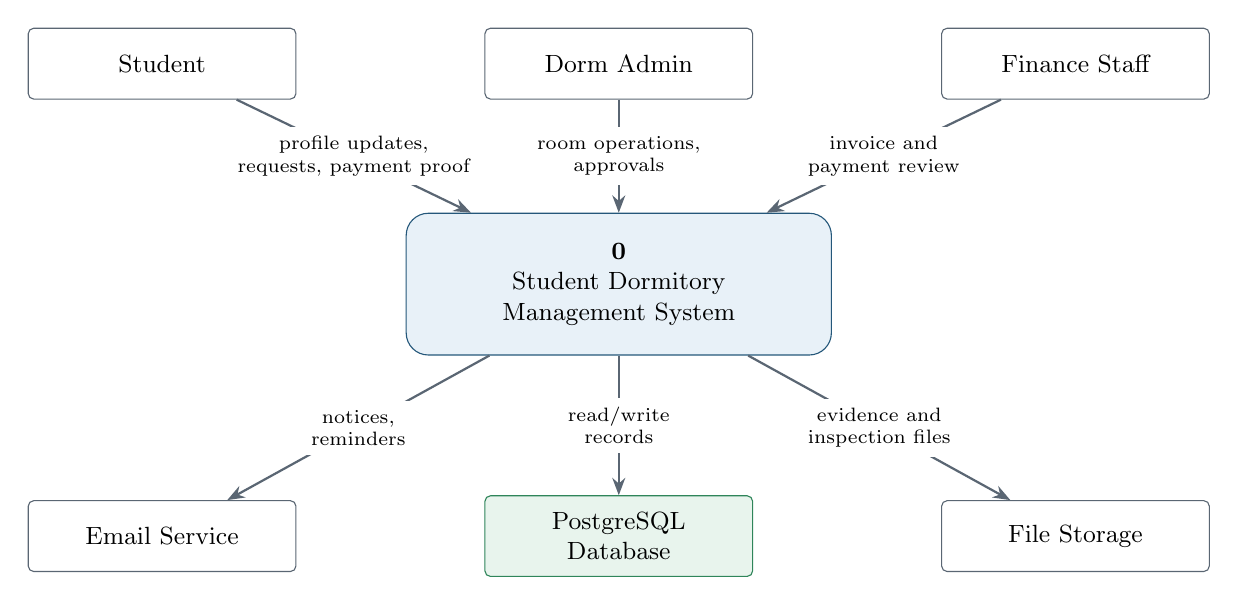
\begin{tikzpicture}[font=\small]
  \node[external, minimum width=34mm] (student) at (0,3.2) {Student};
  \node[external, minimum width=34mm] (admin) at (5.8,3.2) {Dorm Admin};
  \node[external, minimum width=34mm] (finance) at (11.6,3.2) {Finance Staff};

  \node[process, minimum width=54mm, minimum height=18mm] (system) at (5.8,0.4) {\textbf{0}\\Student Dormitory\\Management System};
  \node[external, minimum width=34mm] (email) at (0,-2.8) {Email Service};
  \node[data, minimum width=34mm] (db) at (5.8,-2.8) {PostgreSQL\\Database};
  \node[external, minimum width=34mm] (storage) at (11.6,-2.8) {File Storage};

  \draw[arrow] (student) -- node[fill=white, font=\scriptsize, align=center, midway] {profile updates,\\requests, payment proof} (system);
  \draw[arrow] (admin) -- node[fill=white, font=\scriptsize, align=center, midway] {room operations,\\approvals} (system);
  \draw[arrow] (finance) -- node[fill=white, font=\scriptsize, align=center, midway] {invoice and\\payment review} (system);
  \draw[arrow] (system) -- node[fill=white, font=\scriptsize, align=center, midway] {notices,\\reminders} (email);
  \draw[arrow] (system) -- node[fill=white, font=\scriptsize, align=center, midway] {read/write\\records} (db);
  \draw[arrow] (system) -- node[fill=white, font=\scriptsize, align=center, midway] {evidence and\\inspection files} (storage);
\end{tikzpicture}%
}
\caption{System context diagram}
\end{figure}

\subsection{Assumptions and Constraints}
\begin{itemize}
  \item The MVP is a web application accessed by desktop and mobile browsers.
  \item The first implementation will use Django templates, Bootstrap, HTMX, PostgreSQL, and email integration.
  \item Payment gateway integration is outside the MVP. Students upload evidence, and an authorized staff member confirms payment status.
  \item Synthetic data is acceptable for demo accounts, rooms, invoices, and payments.
  \item Role-based authorization is mandatory for all protected pages and APIs.
\end{itemize}

\section{Requirement Analysis}

\subsection{Functional Requirements}

\begin{longtable}{L{0.11\textwidth} L{0.19\textwidth} L{0.45\textwidth} L{0.10\textwidth}}
\toprule
\textbf{ID} & \textbf{Name} & \textbf{Description} & \textbf{Priority}\\
\midrule
\endhead
FR-01 & Authentication and roles & Users can sign in and access features according to role: Student, Dorm Admin, Finance Staff, and System Administrator. & Must\\
FR-02 & Student profile management & Staff can create, import, update, search, and deactivate student records. Students can view their own profile. & Must\\
FR-03 & Room and bed inventory & Admins can manage buildings, floors, rooms, beds, status, capacity, and occupancy. & Must\\
FR-04 & Automatic assignment & The system recommends or assigns an available bed using policy rules and assignment scoring. & Must\\
FR-05 & Manual assignment override & Admins can manually assign or reassign beds with reason logging. & Should\\
FR-06 & Check-in workflow & Staff can finalize move-in, record handover information, activate the occupancy record, and generate initial charges. & Must\\
FR-07 & Check-out workflow & Staff can record departure request, inspection, penalties, deposit adjustment, and return the bed to inventory. & Must\\
FR-08 & Billing and invoices & Finance staff can generate rent, deposit, fee, and penalty invoices for students. & Must\\
FR-09 & Payment evidence upload & Students can upload payment proof for invoices. The system stores files and links them to payment records. & Must\\
FR-10 & Payment review and confirmation & The system aggregates submitted payment evidence, sends review notification by email, and only authorized staff can confirm paid or rejected status. & Must\\
FR-11 & Notifications and announcements & Admins can broadcast announcements and send reminders for invoices, check-in, check-out, and overdue balances. & Should\\
FR-12 & Dashboard and reports & Staff can view occupancy, available beds, active residents, invoices, payments, and overdue accounts. & Must\\
FR-13 & Audit trail & Critical actions such as assignment, payment confirmation, invoice updates, and check-out settlement are logged. & Should\\
FR-14 & Synthetic demo data & The system can seed realistic demo data for students, rooms, invoices, payments, and occupancy history. & Must\\
\bottomrule
\end{longtable}

\subsection{Non-Functional Requirements}

\begin{longtable}{L{0.14\textwidth} L{0.20\textwidth} L{0.52\textwidth}}
\toprule
\textbf{ID} & \textbf{Quality Attribute} & \textbf{Requirement}\\
\midrule
\endhead
NFR-01 & Security & All protected operations require authentication and role-based authorization. Passwords are hashed. Sensitive records are visible only to permitted roles.\\
NFR-02 & Reliability & Assignment and payment confirmation use database transactions to prevent double booking and inconsistent payment status.\\
NFR-03 & Usability & Common workflows should be completed in a small number of steps, with searchable tables and clear status labels.\\
NFR-04 & Performance & Core list pages should respond within 2 seconds for demo-scale data and remain indexed for larger data.\\
NFR-05 & Maintainability & The codebase should be organized by Django apps and service classes, with business rules separated from views.\\
NFR-06 & Extensibility & Future modules such as visitor management, payment gateways, and university SSO should be addable without rewriting the core model.\\
NFR-07 & Auditability & Financial and occupancy state changes should preserve actor, timestamp, old status, new status, and reason.\\
NFR-08 & Portability & The demo should run locally using environment variables and should support containerized deployment.\\
\bottomrule
\end{longtable}

\subsection{Requirement Prioritization}
The MVP includes the modules needed to run dormitory operations end to end: users, students, rooms, assignment, check-in, billing, payment review, check-out, announcements, dashboard, and demo data. Future enhancements are intentionally kept outside the MVP to reduce implementation risk.

\section{Analysis Models}

\subsection{Use Case Diagram}
The use case model defines the externally visible behavior of the MVP. The system boundary separates user goals from implementation modules. Students mainly consume information and submit evidence or requests; dorm admins operate residence workflows; finance staff control invoices and payment decisions. This separation is important because it drives role-based authorization in the later design.

\begin{figure}[H]
\centering
\resizebox{\textwidth}{!}{%
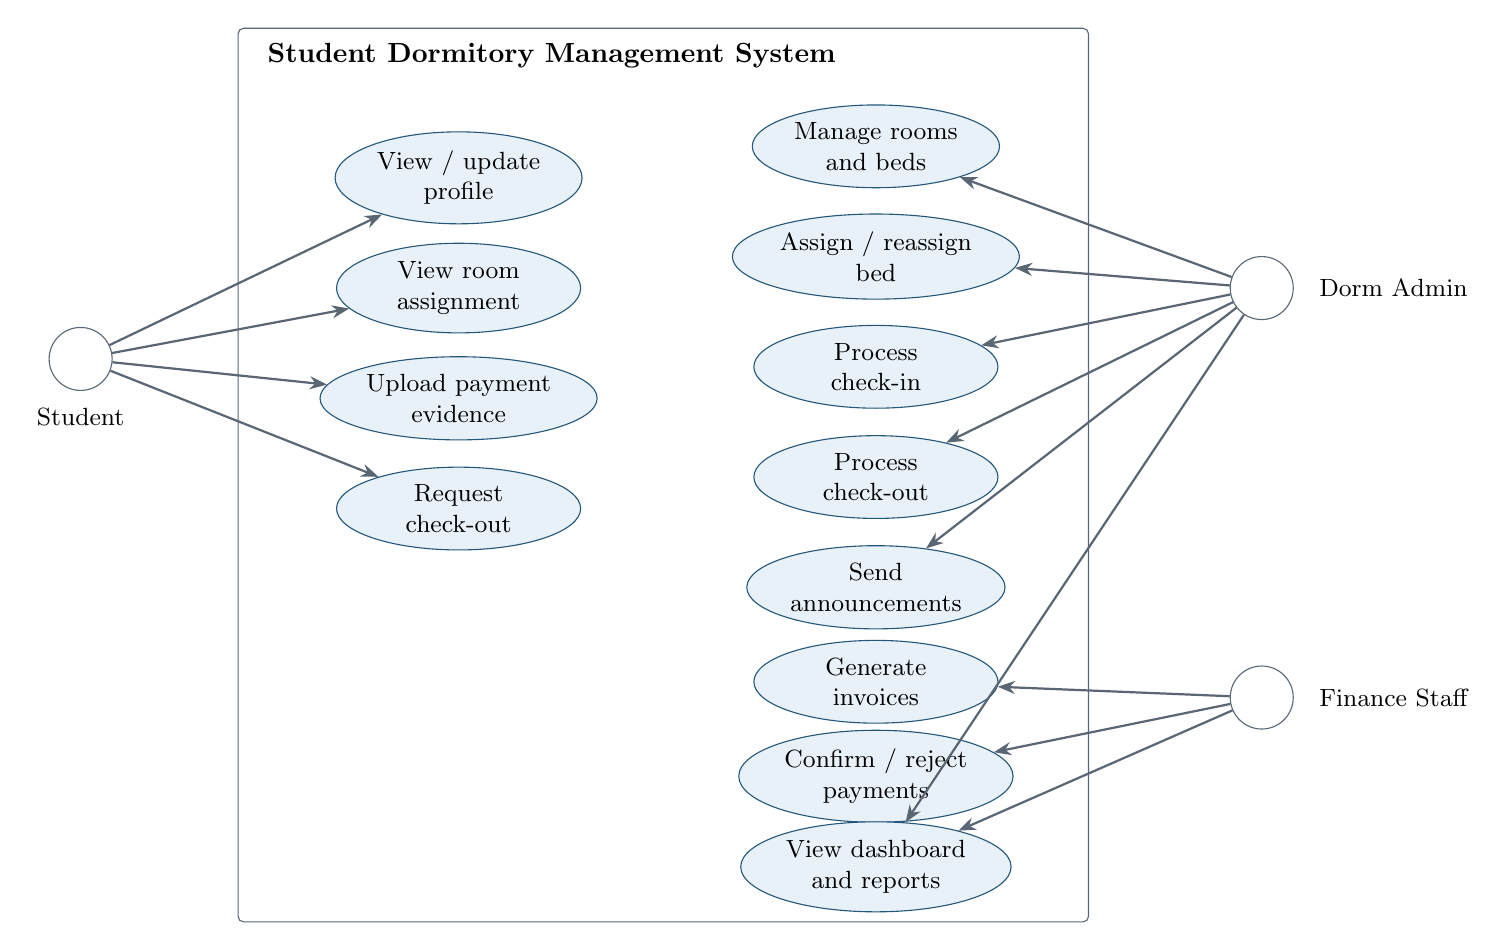
\begin{tikzpicture}[font=\small]
  \draw[draw=linegray, rounded corners=2pt] (2.0,-6.25) rectangle (12.8,5.1);
  \node[anchor=west, font=\bfseries] at (2.25,4.75) {Student Dormitory Management System};

  \node[actor] (student) at (0,0.9) {};
  \node[below=1mm of student] {Student};
  \node[actor] (admin) at (15.0,1.8) {};
  \node[right=2mm of admin] {Dorm Admin};
  \node[actor] (finance) at (15.0,-3.4) {};
  \node[right=2mm of finance] {Finance Staff};

  \node[usecase] (profile) at (4.8,3.2) {View / update\\profile};
  \node[usecase] (assignment) at (4.8,1.8) {View room\\assignment};
  \node[usecase] (payupload) at (4.8,0.4) {Upload payment\\evidence};
  \node[usecase] (checkoutreq) at (4.8,-1.0) {Request\\check-out};

  \node[usecase] (rooms) at (10.1,3.6) {Manage rooms\\and beds};
  \node[usecase] (assign) at (10.1,2.2) {Assign / reassign\\bed};
  \node[usecase] (checkin) at (10.1,0.8) {Process\\check-in};
  \node[usecase] (checkout) at (10.1,-0.6) {Process\\check-out};
  \node[usecase] (announce) at (10.1,-2.0) {Send\\announcements};
  \node[usecase] (billing) at (10.1,-3.2) {Generate\\invoices};
  \node[usecase] (confirm) at (10.1,-4.4) {Confirm / reject\\payments};
  \node[usecase] (reports) at (10.1,-5.55) {View dashboard\\and reports};

  \draw[arrow] (student) -- (profile);
  \draw[arrow] (student) -- (assignment);
  \draw[arrow] (student) -- (payupload);
  \draw[arrow] (student) -- (checkoutreq);

  \draw[arrow] (admin) -- (rooms);
  \draw[arrow] (admin) -- (assign);
  \draw[arrow] (admin) -- (checkin);
  \draw[arrow] (admin) -- (checkout);
  \draw[arrow] (admin) -- (announce);
  \draw[arrow] (admin) -- (reports);

  \draw[arrow] (finance) -- (billing);
  \draw[arrow] (finance) -- (confirm);
  \draw[arrow] (finance) -- (reports);
\end{tikzpicture}%
}
\caption{Use case diagram for the MVP}
\end{figure}

The use case diagram also identifies authorization boundaries. For example, a student can upload evidence but cannot confirm a payment. Finance can confirm payments but should not directly change room inventory. Those boundaries later become permission decorators, navigation rules, and negative tests.

\subsection{Activity Diagrams}
Activity diagrams describe workflow ordering and decision points. They are used here for the three workflows most likely to create inconsistent data if implemented incorrectly: onboarding, payment review, and check-out settlement.

\subsubsection*{Student Onboarding and Assignment}
The onboarding activity starts from a student record and ends with an active occupancy record. The key decision points are bed availability and payment confirmation. If no bed is available, the student enters a waiting-list path. If payment is not confirmed, the system sends reminders and does not activate the bed.

\begin{figure}[H]
\centering
\resizebox{0.92\textwidth}{!}{%
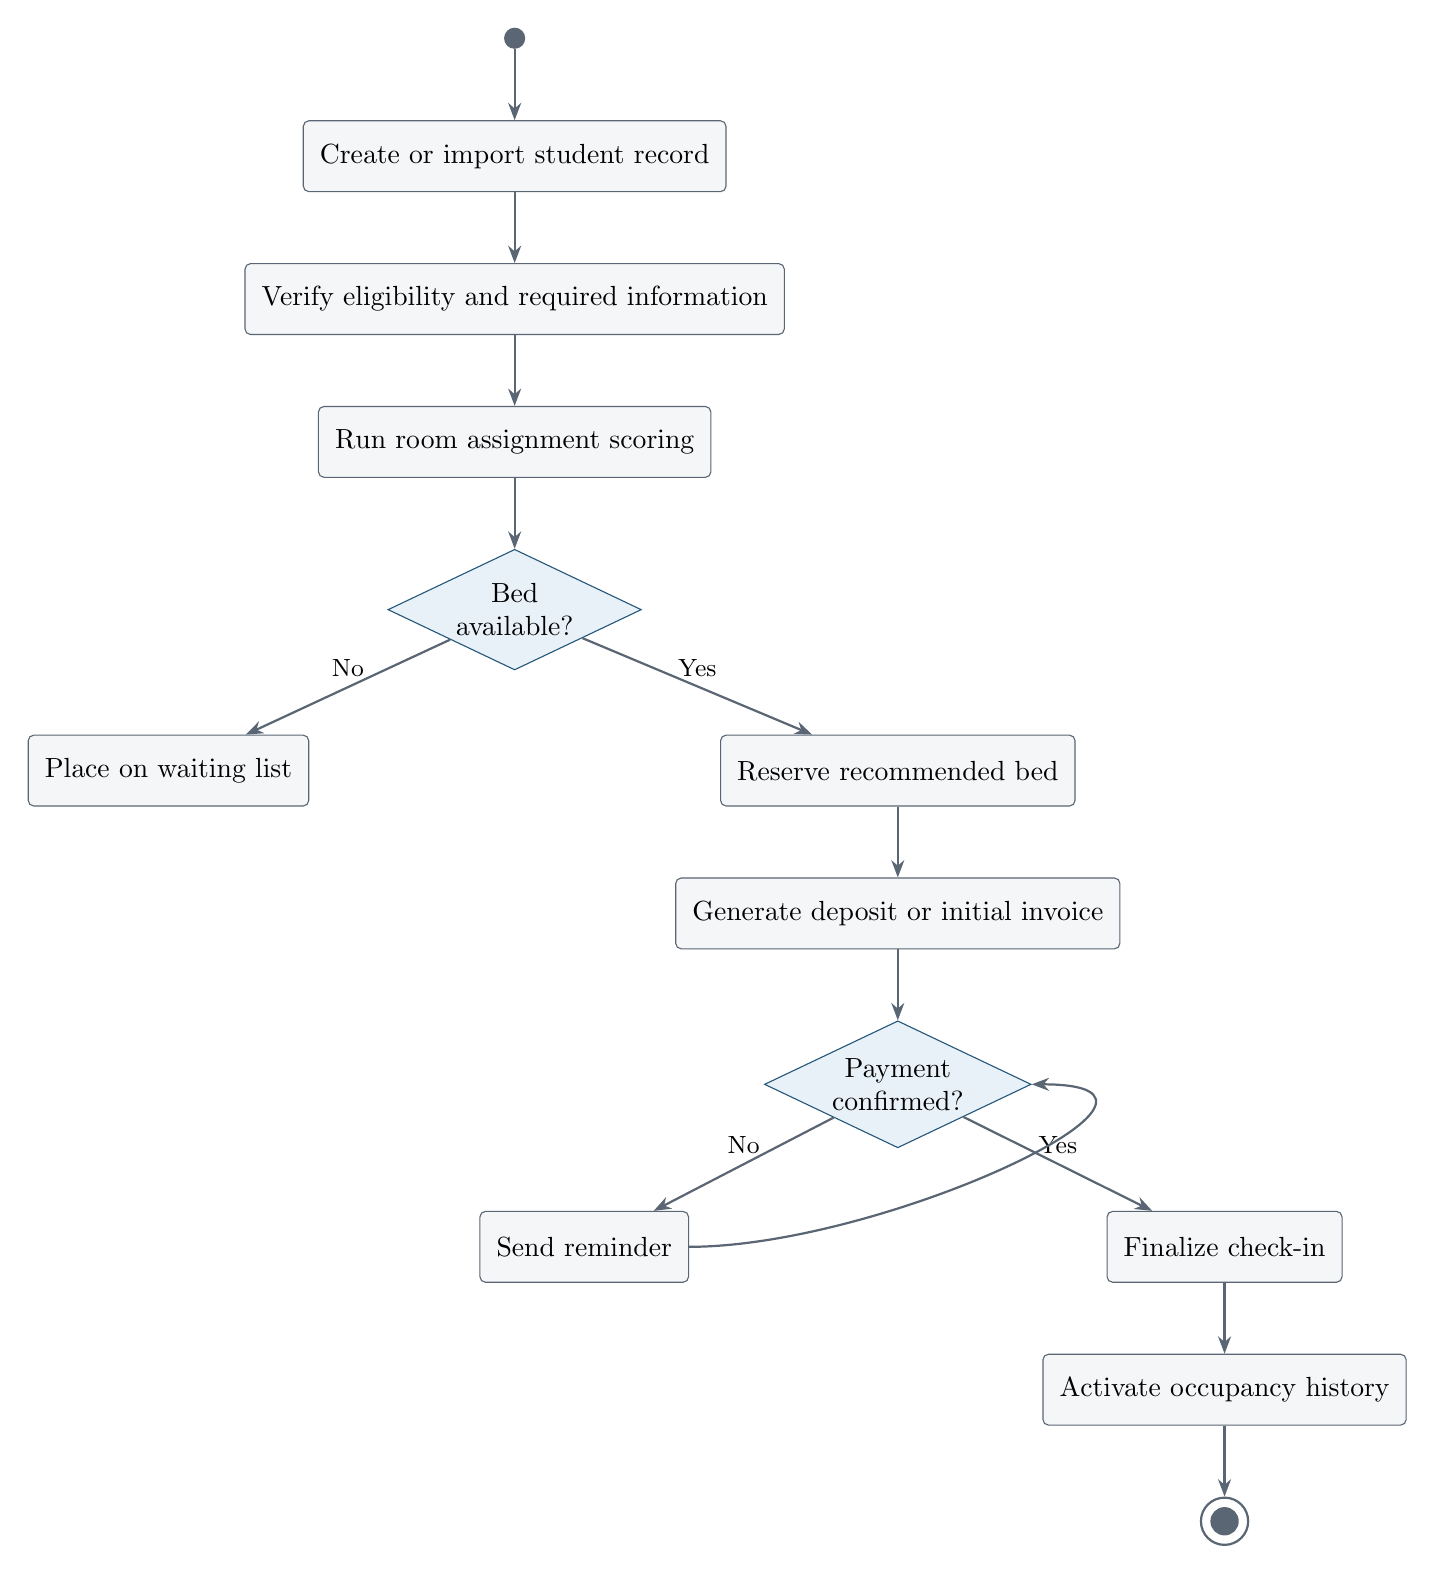
\begin{tikzpicture}[node distance=9mm]
  \node[circle, fill=linegray, inner sep=2.7pt] (start) {};
  \node[box, below=of start] (record) {Create or import student record};
  \node[box, below=of record] (elig) {Verify eligibility and required information};
  \node[box, below=of elig] (score) {Run room assignment scoring};
  \node[decision, below=of score] (available) {Bed\\available?};
  \node[box, below left=12mm and 18mm of available] (waitlist) {Place on waiting list};
  \node[box, below right=12mm and 18mm of available] (reserve) {Reserve recommended bed};
  \node[box, below=of reserve] (invoice) {Generate deposit or initial invoice};
  \node[decision, below=of invoice] (paid) {Payment\\confirmed?};
  \node[box, below left=12mm and 18mm of paid] (reminder) {Send reminder};
  \node[box, below right=12mm and 18mm of paid] (checkin) {Finalize check-in};
  \node[box, below=of checkin] (active) {Activate occupancy history};
  \node[circle, draw=linegray, thick, minimum size=6mm, below=of active] (end) {};
  \fill[linegray] (end.center) circle (1.8mm);

  \draw[arrow] (start) -- (record);
  \draw[arrow] (record) -- (elig);
  \draw[arrow] (elig) -- (score);
  \draw[arrow] (score) -- (available);
  \draw[arrow] (available) -- node[above, font=\small] {No} (waitlist);
  \draw[arrow] (available) -- node[above, font=\small] {Yes} (reserve);
  \draw[arrow] (reserve) -- (invoice);
  \draw[arrow] (invoice) -- (paid);
  \draw[arrow] (paid) -- node[above, font=\small] {No} (reminder);
  \draw[arrow] (paid) -- node[above, font=\small] {Yes} (checkin);
  \draw[arrow] (reminder.east) .. controls +(25mm,0) and +(25mm,0) .. (paid.east);
  \draw[arrow] (checkin) -- (active);
  \draw[arrow] (active) -- (end);
\end{tikzpicture}%
}
\caption{Activity diagram for onboarding}
\end{figure}

\subsubsection*{Payment Evidence Review}
The payment workflow is intentionally two-step: students submit evidence, while finance staff make the financial decision. Pending evidence does not reduce outstanding balance. This protects the receivable record from accidental or fraudulent student-side updates.

\begin{figure}[H]
\centering
\resizebox{0.96\textwidth}{!}{%
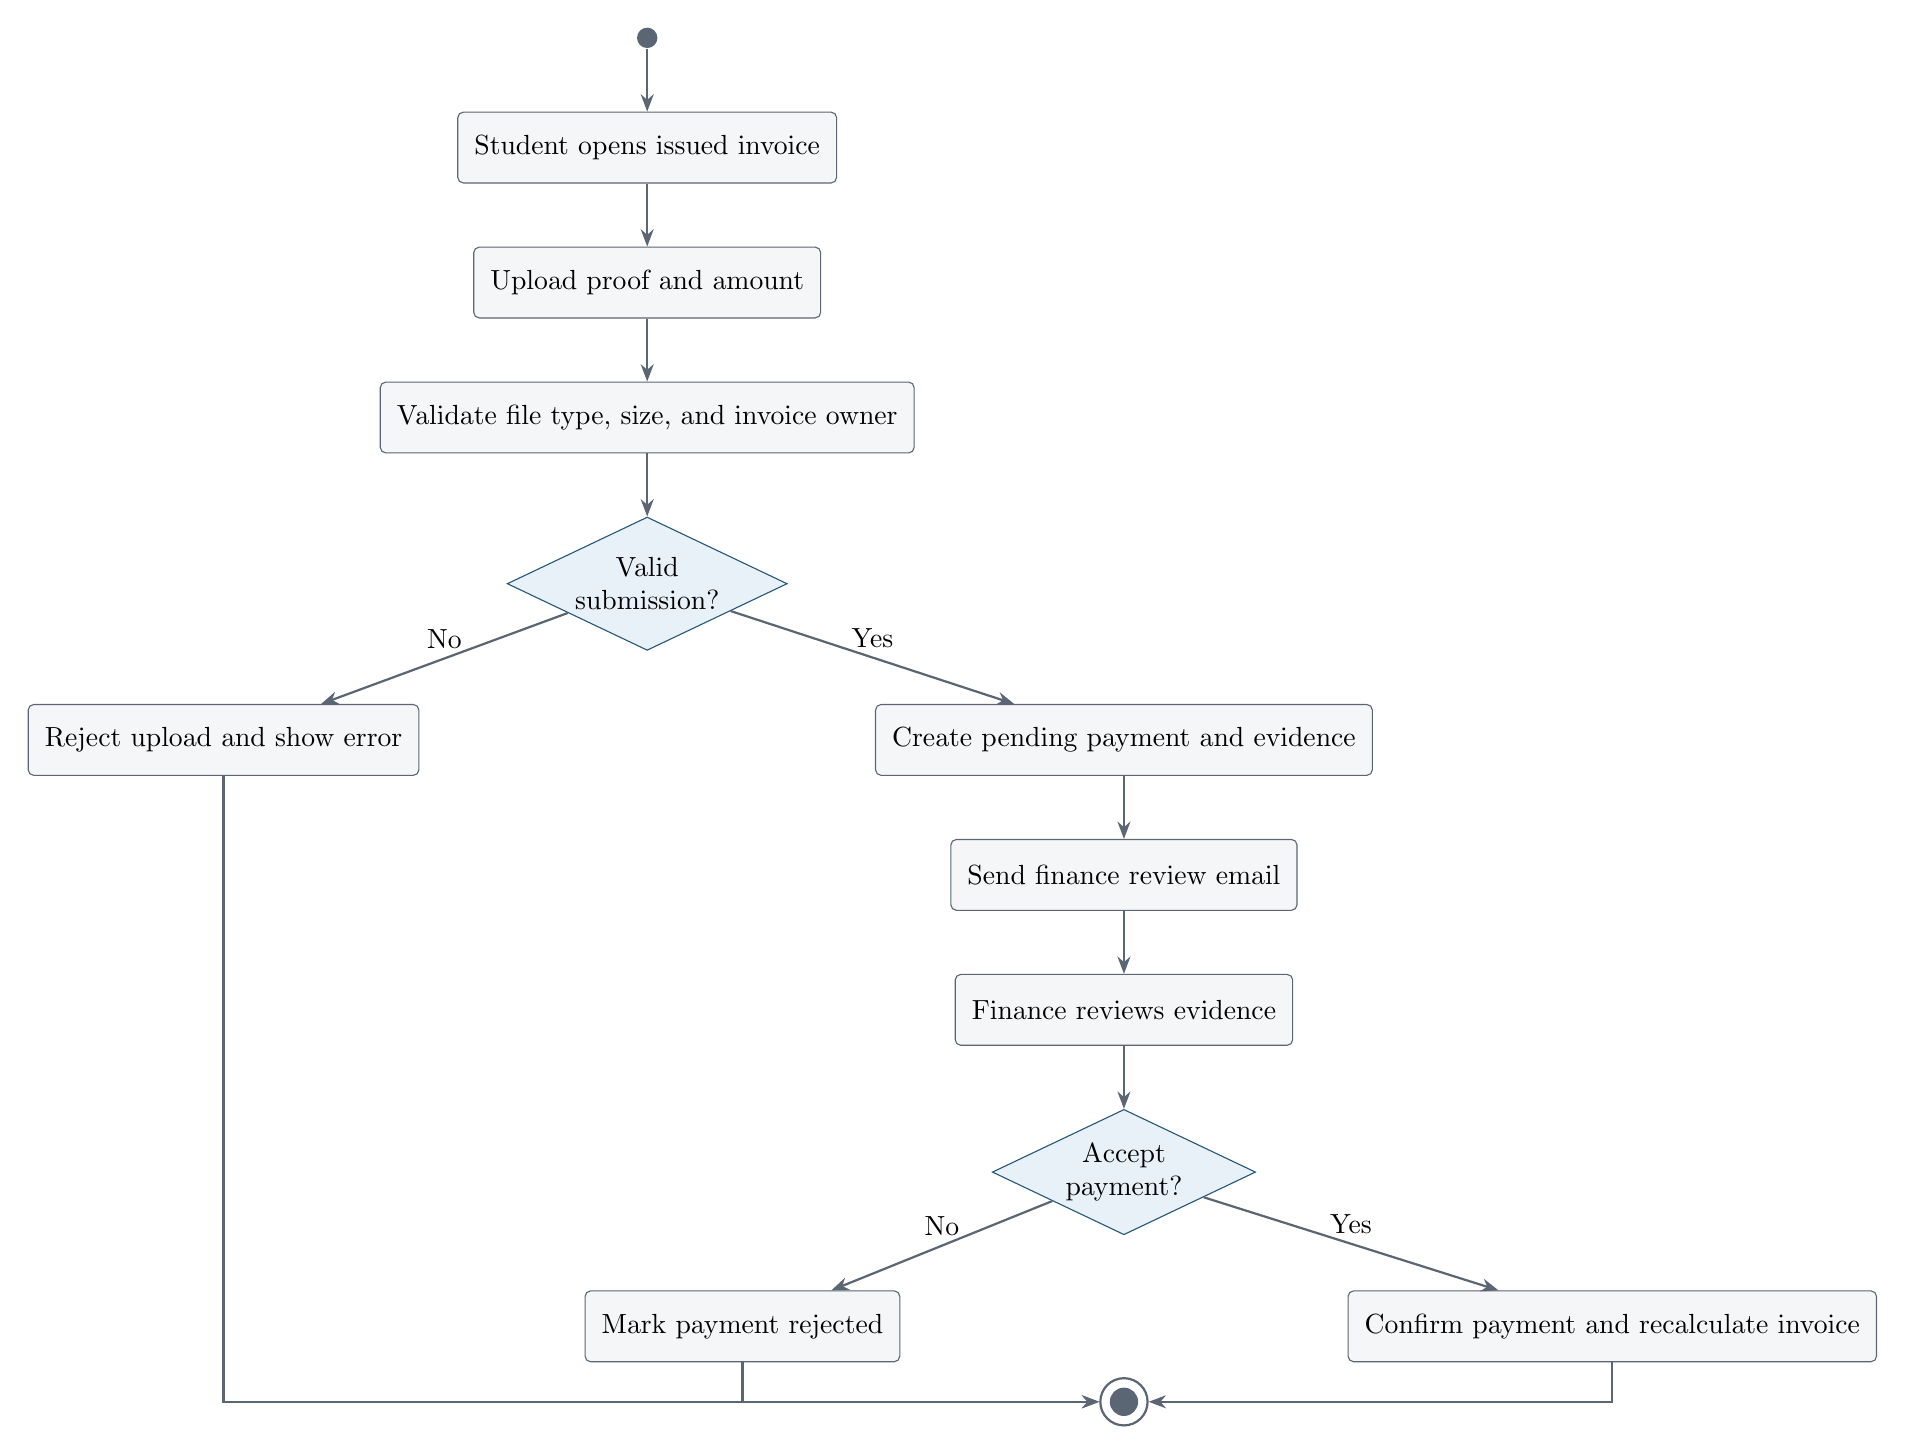
\begin{tikzpicture}[node distance=8mm]
  \node[circle, fill=linegray, inner sep=2.6pt] (start) {};
  \node[box, below=of start] (invoice) {Student opens issued invoice};
  \node[box, below=of invoice] (upload) {Upload proof and amount};
  \node[box, below=of upload] (validate) {Validate file type, size, and invoice owner};
  \node[decision, below=of validate] (valid) {Valid\\submission?};
  \node[box, below left=11mm and 20mm of valid] (rejectfile) {Reject upload and show error};
  \node[box, below right=11mm and 20mm of valid] (pending) {Create pending payment and evidence};
  \node[box, below=of pending] (email) {Send finance review email};
  \node[box, below=of email] (review) {Finance reviews evidence};
  \node[decision, below=of review] (decision) {Accept\\payment?};
  \node[box, below left=11mm and 20mm of decision] (rejectpay) {Mark payment rejected};
  \node[box, below right=11mm and 20mm of decision] (confirm) {Confirm payment and recalculate invoice};
  \node[circle, draw=linegray, thick, minimum size=6mm, below=18mm of decision] (end) {};
  \fill[linegray] (end.center) circle (1.8mm);

  \draw[arrow] (start) -- (invoice);
  \draw[arrow] (invoice) -- (upload);
  \draw[arrow] (upload) -- (validate);
  \draw[arrow] (validate) -- (valid);
  \draw[arrow] (valid) -- node[above] {No} (rejectfile);
  \draw[arrow] (valid) -- node[above] {Yes} (pending);
  \draw[arrow] (pending) -- (email);
  \draw[arrow] (email) -- (review);
  \draw[arrow] (review) -- (decision);
  \draw[arrow] (decision) -- node[above] {No} (rejectpay);
  \draw[arrow] (decision) -- node[above] {Yes} (confirm);
  \draw[arrow] (rejectfile.south) |- (end.west);
  \draw[arrow] (rejectpay.south) |- (end.west);
  \draw[arrow] (confirm.south) |- (end.east);
\end{tikzpicture}%
}
\caption{Activity diagram for payment evidence review}
\end{figure}

\subsubsection*{Check-out Settlement}
The check-out activity coordinates operations and finance. It records inspection data, calculates damage fees and unpaid balances, updates deposit settlement, and releases or blocks the bed depending on the inspection result.

\begin{figure}[H]
\centering
\resizebox{0.96\textwidth}{!}{%
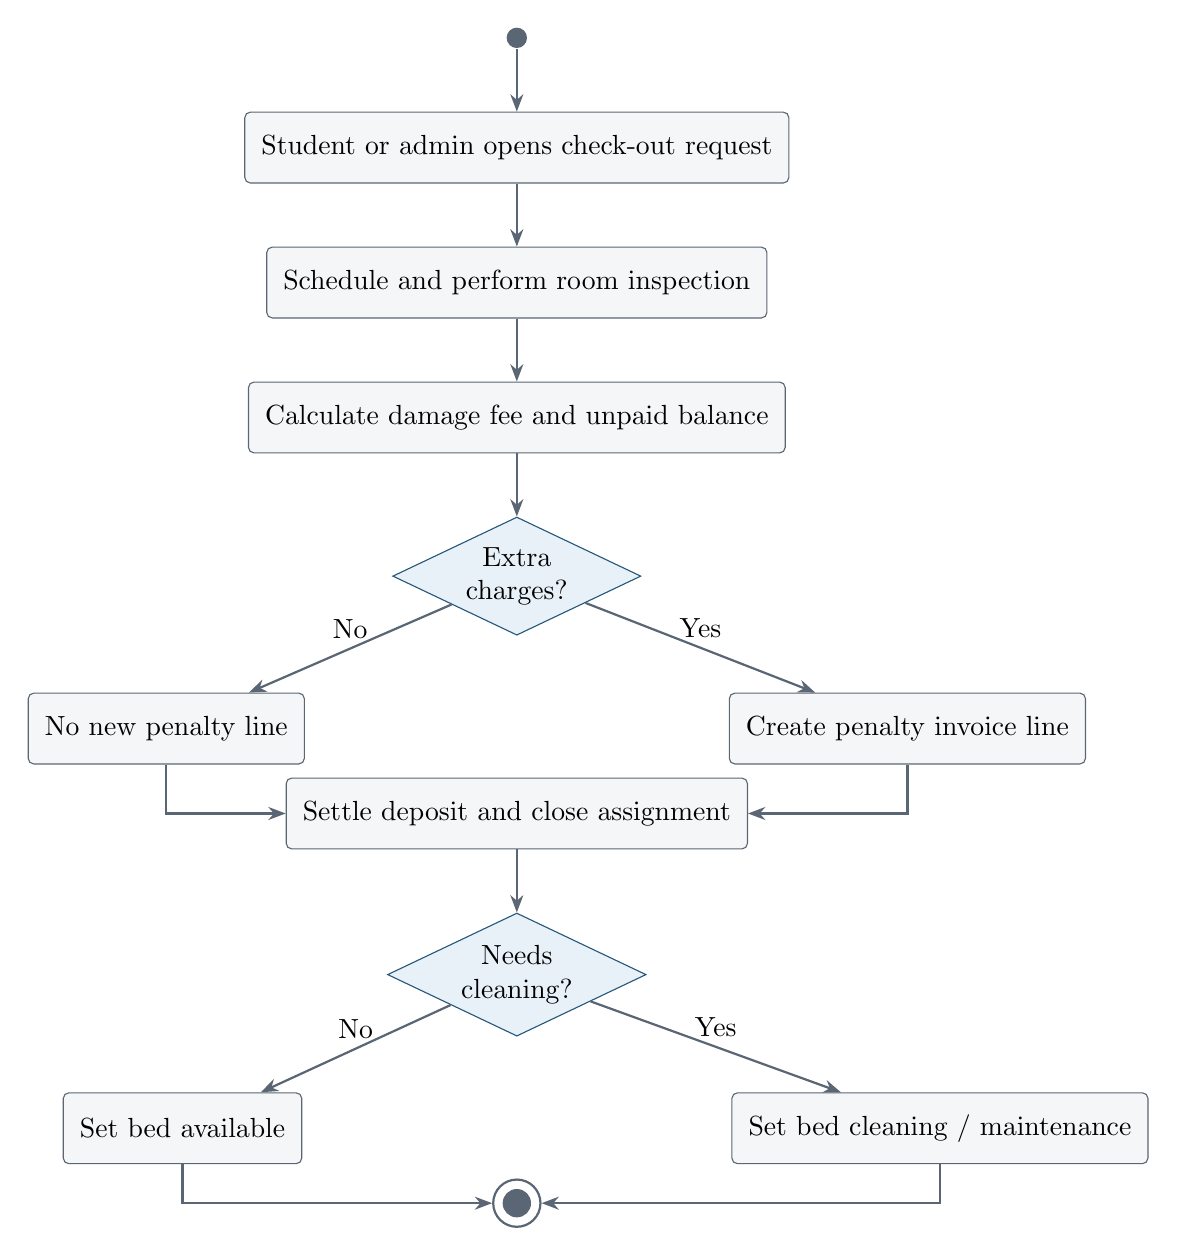
\begin{tikzpicture}[node distance=8mm]
  \node[circle, fill=linegray, inner sep=2.6pt] (start) {};
  \node[box, below=of start] (request) {Student or admin opens check-out request};
  \node[box, below=of request] (schedule) {Schedule and perform room inspection};
  \node[box, below=of schedule] (fees) {Calculate damage fee and unpaid balance};
  \node[decision, below=of fees] (charges) {Extra\\charges?};
  \node[box, below left=11mm and 19mm of charges] (none) {No new penalty line};
  \node[box, below right=11mm and 19mm of charges] (penalty) {Create penalty invoice line};
  \node[box, below=18mm of charges] (settle) {Settle deposit and close assignment};
  \node[decision, below=of settle] (clean) {Needs\\cleaning?};
  \node[box, below left=11mm and 19mm of clean] (available) {Set bed available};
  \node[box, below right=11mm and 19mm of clean] (cleaning) {Set bed cleaning / maintenance};
  \node[circle, draw=linegray, thick, minimum size=6mm, below=18mm of clean] (end) {};
  \fill[linegray] (end.center) circle (1.8mm);

  \draw[arrow] (start) -- (request);
  \draw[arrow] (request) -- (schedule);
  \draw[arrow] (schedule) -- (fees);
  \draw[arrow] (fees) -- (charges);
  \draw[arrow] (charges) -- node[above] {No} (none);
  \draw[arrow] (charges) -- node[above] {Yes} (penalty);
  \draw[arrow] (none.south) |- (settle.west);
  \draw[arrow] (penalty.south) |- (settle.east);
  \draw[arrow] (settle) -- (clean);
  \draw[arrow] (clean) -- node[above] {No} (available);
  \draw[arrow] (clean) -- node[above] {Yes} (cleaning);
  \draw[arrow] (available.south) |- (end.west);
  \draw[arrow] (cleaning.south) |- (end.east);
\end{tikzpicture}%
}
\caption{Activity diagram for check-out settlement}
\end{figure}

\subsection{Sequence Diagrams}
Sequence diagrams show the same workflows from a runtime collaboration perspective. They clarify which component owns validation, transaction control, file storage, email sending, and state updates.

\subsubsection*{Bed Reservation and Check-in}
The reservation sequence shows why bed assignment must be implemented in a service transaction. The bed row is locked before the assignment is created so two admins cannot reserve the same bed concurrently.

\begin{figure}[H]
\centering
\resizebox{\textwidth}{!}{%
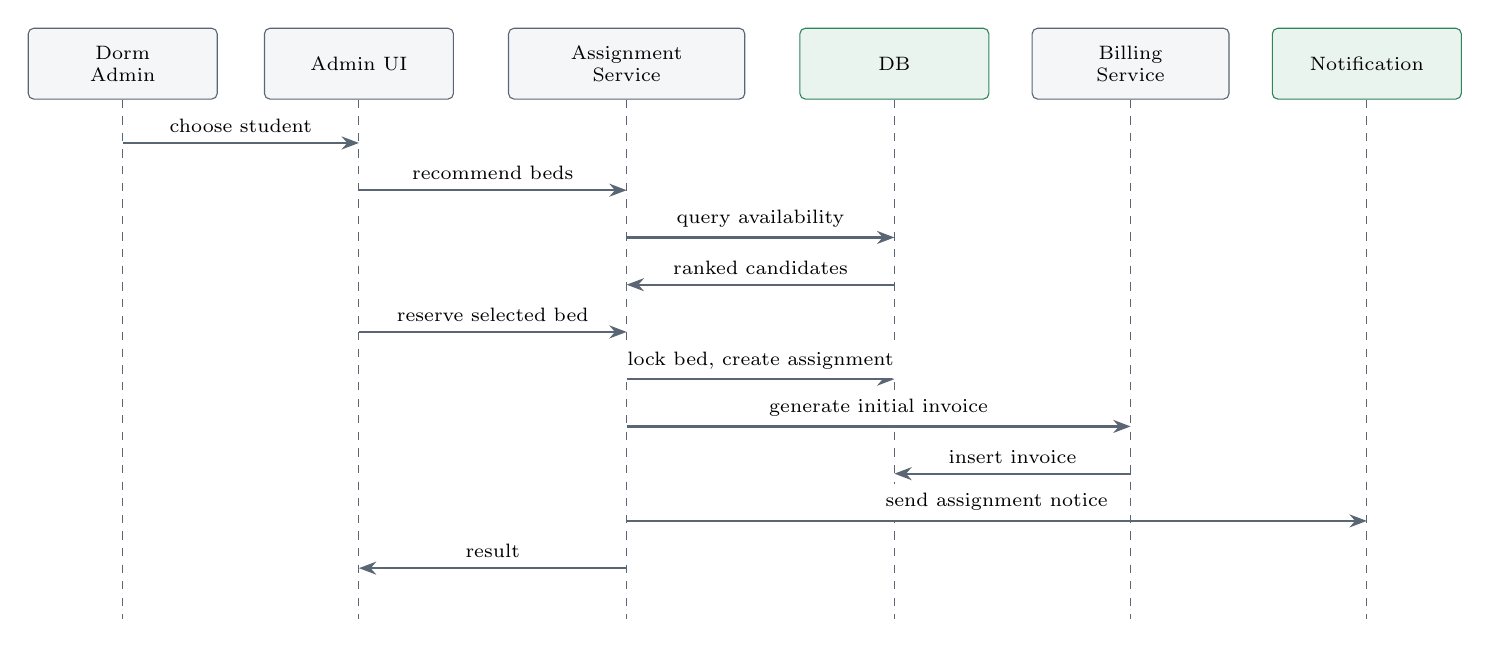
\begin{tikzpicture}[font=\scriptsize]
  \node[box, minimum width=24mm] (admin) at (0,0) {Dorm\\Admin};
  \node[box, minimum width=24mm] (ui) at (3.0,0) {Admin UI};
  \node[box, minimum width=30mm] (svc) at (6.4,0) {Assignment\\Service};
  \node[data, minimum width=24mm] (db) at (9.8,0) {DB};
  \node[box, minimum width=25mm] (bill) at (12.8,0) {Billing\\Service};
  \node[data, minimum width=24mm] (notify) at (15.8,0) {Notification};

  \foreach \x in {admin,ui,svc,db,bill,notify} {
    \draw[dashed, draw=linegray] (\x.south) -- ++(0,-6.6);
  }

  \draw[arrow] (admin.south) ++(0,-0.55) -- node[above, fill=white] {choose student} ($(ui.south)+(0,-0.55)$);
  \draw[arrow] (ui.south) ++(0,-1.15) -- node[above, fill=white] {recommend beds} ($(svc.south)+(0,-1.15)$);
  \draw[arrow] (svc.south) ++(0,-1.75) -- node[above, fill=white] {query availability} ($(db.south)+(0,-1.75)$);
  \draw[arrow] (db.south) ++(0,-2.35) -- node[above, fill=white] {ranked candidates} ($(svc.south)+(0,-2.35)$);
  \draw[arrow] (ui.south) ++(0,-2.95) -- node[above, fill=white] {reserve selected bed} ($(svc.south)+(0,-2.95)$);
  \draw[arrow] (svc.south) ++(0,-3.55) -- node[above, fill=white] {lock bed, create assignment} ($(db.south)+(0,-3.55)$);
  \draw[arrow] (svc.south) ++(0,-4.15) -- node[above, fill=white] {generate initial invoice} ($(bill.south)+(0,-4.15)$);
  \draw[arrow] (bill.south) ++(0,-4.75) -- node[above, fill=white] {insert invoice} ($(db.south)+(0,-4.75)$);
  \draw[arrow] (svc.south) ++(0,-5.35) -- node[above, fill=white] {send assignment notice} ($(notify.south)+(0,-5.35)$);
  \draw[arrow] (svc.south) ++(0,-5.95) -- node[above, fill=white] {result} ($(ui.south)+(0,-5.95)$);
\end{tikzpicture}%
}
\caption{Sequence diagram for bed reservation and check-in preparation}
\end{figure}

\subsubsection*{Payment Evidence Review}
This sequence separates file storage from database state. The system first validates invoice ownership, stores the evidence file, creates a pending payment, and then asks finance to review. Only the final finance decision updates the invoice balance.

\begin{figure}[H]
\centering
\resizebox{\textwidth}{!}{%
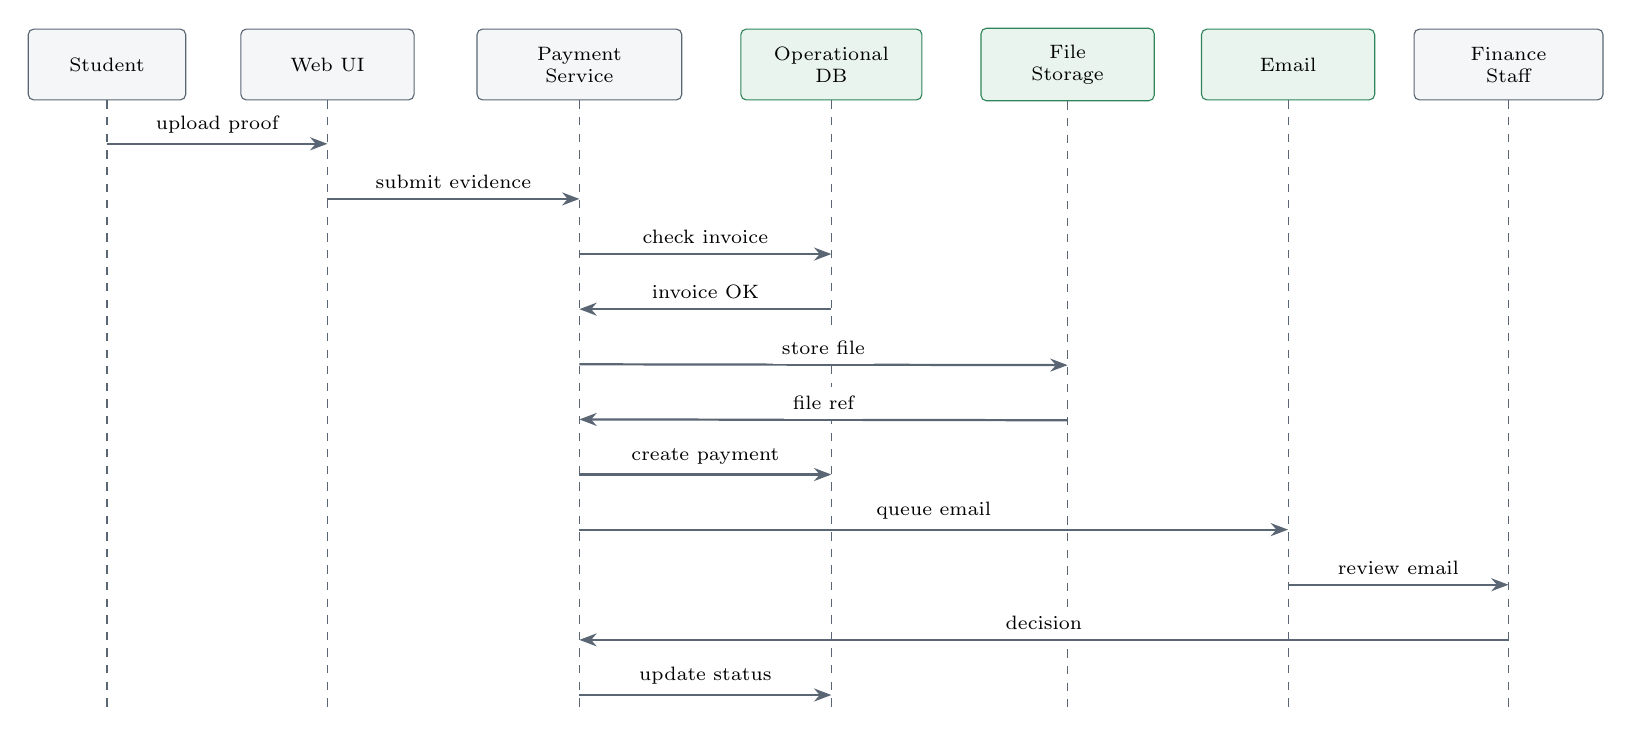
\begin{tikzpicture}[font=\scriptsize]
  \node[box, minimum width=20mm] (student) at (0,0) {Student};
  \node[box, minimum width=22mm] (web) at (2.8,0) {Web UI};
  \node[box, minimum width=26mm] (pay) at (6.0,0) {Payment\\Service};
  \node[data, minimum width=23mm] (db) at (9.2,0) {Operational\\DB};
  \node[data, minimum width=22mm] (store) at (12.2,0) {File\\Storage};
  \node[data, minimum width=22mm] (email) at (15.0,0) {Email};
  \node[box, minimum width=24mm] (finance) at (17.8,0) {Finance\\Staff};

  \foreach \x in {student,web,pay,db,store,email,finance} {
    \draw[dashed, draw=linegray] (\x.south) -- ++(0,-7.8);
  }

  \draw[arrow] (student.south) ++(0,-0.55) -- node[above, fill=white] {upload proof} ($(web.south)+(0,-0.55)$);
  \draw[arrow] (web.south) ++(0,-1.25) -- node[above, fill=white] {submit evidence} ($(pay.south)+(0,-1.25)$);
  \draw[arrow] (pay.south) ++(0,-1.95) -- node[above, fill=white] {check invoice} ($(db.south)+(0,-1.95)$);
  \draw[arrow] (db.south) ++(0,-2.65) -- node[above, fill=white] {invoice OK} ($(pay.south)+(0,-2.65)$);
  \draw[arrow] (pay.south) ++(0,-3.35) -- node[above, fill=white] {store file} ($(store.south)+(0,-3.35)$);
  \draw[arrow] (store.south) ++(0,-4.05) -- node[above, fill=white] {file ref} ($(pay.south)+(0,-4.05)$);
  \draw[arrow] (pay.south) ++(0,-4.75) -- node[above, fill=white] {create payment} ($(db.south)+(0,-4.75)$);
  \draw[arrow] (pay.south) ++(0,-5.45) -- node[above, fill=white] {queue email} ($(email.south)+(0,-5.45)$);
  \draw[arrow] (email.south) ++(0,-6.15) -- node[above, fill=white] {review email} ($(finance.south)+(0,-6.15)$);
  \draw[arrow] (finance.south) ++(0,-6.85) -- node[above, fill=white] {decision} ($(pay.south)+(0,-6.85)$);
  \draw[arrow] (pay.south) ++(0,-7.55) -- node[above, fill=white] {update status} ($(db.south)+(0,-7.55)$);
\end{tikzpicture}%
}
\caption{Sequence diagram for payment evidence review}
\end{figure}

\subsubsection*{Check-out Settlement}
The check-out sequence shows that checkout is not just a bed status update. It joins inspection, billing, deposit adjustment, assignment closure, and audit logging in one transactional service operation.

\begin{figure}[H]
\centering
\resizebox{\textwidth}{!}{%
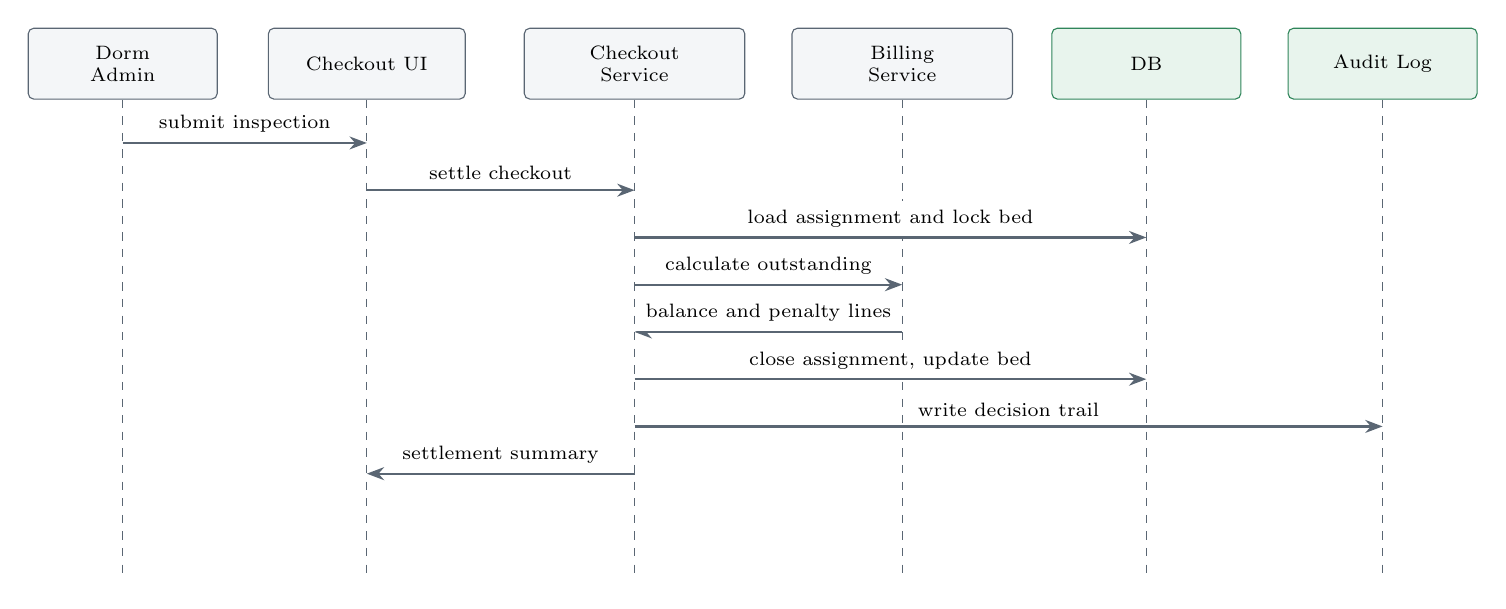
\begin{tikzpicture}[font=\scriptsize]
  \node[box, minimum width=24mm] (admin) at (0,0) {Dorm\\Admin};
  \node[box, minimum width=25mm] (ui) at (3.1,0) {Checkout UI};
  \node[box, minimum width=28mm] (svc) at (6.5,0) {Checkout\\Service};
  \node[box, minimum width=28mm] (bill) at (9.9,0) {Billing\\Service};
  \node[data, minimum width=24mm] (db) at (13.0,0) {DB};
  \node[data, minimum width=24mm] (audit) at (16.0,0) {Audit Log};

  \foreach \x in {admin,ui,svc,bill,db,audit} {
    \draw[dashed, draw=linegray] (\x.south) -- ++(0,-6.1);
  }

  \draw[arrow] (admin.south) ++(0,-0.55) -- node[above, fill=white] {submit inspection} ($(ui.south)+(0,-0.55)$);
  \draw[arrow] (ui.south) ++(0,-1.15) -- node[above, fill=white] {settle checkout} ($(svc.south)+(0,-1.15)$);
  \draw[arrow] (svc.south) ++(0,-1.75) -- node[above, fill=white] {load assignment and lock bed} ($(db.south)+(0,-1.75)$);
  \draw[arrow] (svc.south) ++(0,-2.35) -- node[above, fill=white] {calculate outstanding} ($(bill.south)+(0,-2.35)$);
  \draw[arrow] (bill.south) ++(0,-2.95) -- node[above, fill=white] {balance and penalty lines} ($(svc.south)+(0,-2.95)$);
  \draw[arrow] (svc.south) ++(0,-3.55) -- node[above, fill=white] {close assignment, update bed} ($(db.south)+(0,-3.55)$);
  \draw[arrow] (svc.south) ++(0,-4.15) -- node[above, fill=white] {write decision trail} ($(audit.south)+(0,-4.15)$);
  \draw[arrow] (svc.south) ++(0,-4.75) -- node[above, fill=white] {settlement summary} ($(ui.south)+(0,-4.75)$);
\end{tikzpicture}%
}
\caption{Sequence diagram for check-out settlement}
\end{figure}

\subsection{State Diagrams}
State diagrams define legal lifecycle transitions. They are the basis for validation functions such as \texttt{set\_bed\_status}, \texttt{confirm\_payment}, and \texttt{settle\_checkout}.

\subsubsection*{Bed Lifecycle}
The bed lifecycle prevents double booking. Only available beds can be reserved, only reserved beds can become occupied, and check-out moves the bed either back to available or into cleaning/maintenance.

\begin{figure}[H]
\centering
\resizebox{\textwidth}{!}{%
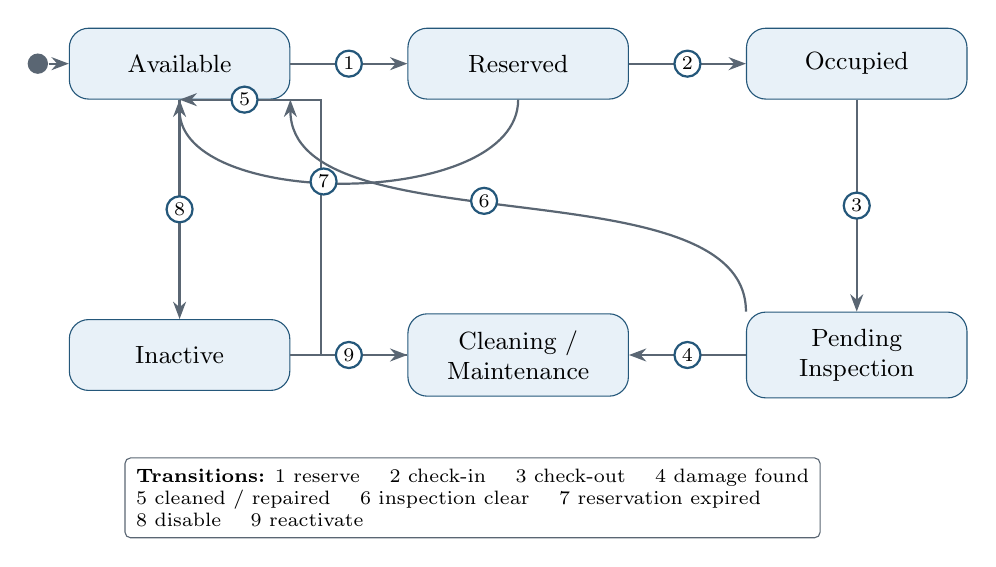
\begin{tikzpicture}[font=\small]
  \tikzset{stag/.style={circle, draw=primary, fill=white, inner sep=1.2pt, font=\scriptsize}}
  \node[circle, fill=linegray, inner sep=2.6pt] (init) at (-1.1,2.0) {};
  \node[state] (available) at (0.7,2.0) {Available};
  \node[state] (reserved) at (5.0,2.0) {Reserved};
  \node[state] (occupied) at (9.3,2.0) {Occupied};
  \node[state] (inactive) at (0.7,-1.7) {Inactive};
  \node[state] (cleaning) at (5.0,-1.7) {Cleaning /\\Maintenance};
  \node[state] (inspection) at (9.3,-1.7) {Pending\\Inspection};

  \draw[arrow] (init) -- (available);
  \draw[arrow] (available) -- node[stag, midway] {1} (reserved);
  \draw[arrow] (reserved) -- node[stag, midway] {2} (occupied);
  \draw[arrow] (occupied) -- node[stag, midway] {3} (inspection);
  \draw[arrow] (inspection) -- node[stag, midway] {4} (cleaning);
  \draw[arrow] (cleaning.west) -- ++(-1.1,0) |- node[stag, pos=0.77] {5} (available.south);
  \draw[arrow] (inspection.north west) .. controls +(0,19mm) and +(0,-19mm) .. node[stag, pos=0.55] {6} (available.south east);
  \draw[arrow] (reserved.south) .. controls +(0,-14mm) and +(0,-14mm) .. node[stag, pos=0.55] {7} (available.south);
  \draw[arrow] (available) -- node[stag, midway] {8} (inactive);
  \draw[arrow] (inactive) -- node[stag, midway] {9} (cleaning);

  \node[draw=linegray, fill=white, rounded corners=2pt, align=left, inner sep=4pt, anchor=north west, font=\scriptsize] at (0.0,-3.0) {
    \textbf{Transitions:}
    1 reserve \quad 2 check-in \quad 3 check-out \quad 4 damage found\\
    5 cleaned / repaired \quad 6 inspection clear \quad 7 reservation expired\\
    8 disable \quad 9 reactivate
  };
\end{tikzpicture}%
}
\caption{State diagram for a bed}
\end{figure}

\subsubsection*{Assignment Lifecycle}
The assignment state controls resident history. A canceled or completed assignment remains as historical evidence, while transfer creates a new assignment record instead of overwriting the old one.

\begin{figure}[H]
\centering
\resizebox{0.86\textwidth}{!}{%
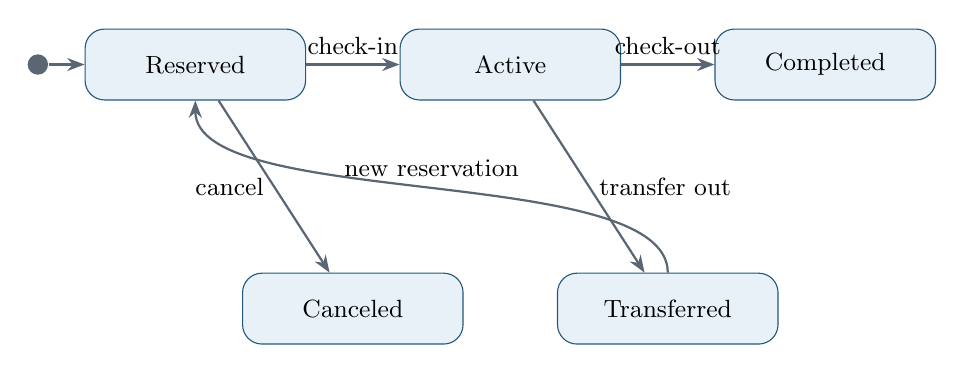
\begin{tikzpicture}[font=\small]
  \node[circle, fill=linegray, inner sep=2.6pt] (init) at (-1,1.4) {};
  \node[state] (reserved) at (1.0,1.4) {Reserved};
  \node[state] (active) at (5.0,1.4) {Active};
  \node[state] (completed) at (9.0,1.4) {Completed};
  \node[state] (cancelled) at (3.0,-1.7) {Canceled};
  \node[state] (transferred) at (7.0,-1.7) {Transferred};

  \draw[arrow] (init) -- (reserved);
  \draw[arrow] (reserved) -- node[above] {check-in} (active);
  \draw[arrow] (active) -- node[above] {check-out} (completed);
  \draw[arrow] (reserved) -- node[left] {cancel} (cancelled);
  \draw[arrow] (active) -- node[right] {transfer out} (transferred);
  \draw[arrow] (transferred.north) .. controls +(0,14mm) and +(0,-14mm) .. node[above] {new reservation} (reserved.south);
\end{tikzpicture}%
}
\caption{State diagram for an assignment}
\end{figure}

\subsubsection*{Payment Lifecycle}
The payment lifecycle ensures that uploaded evidence is not treated as money until finance approves it. Confirmed payments can settle invoices; rejected payments remain visible for audit and student feedback.

\begin{figure}[H]
\centering
\resizebox{0.82\textwidth}{!}{%
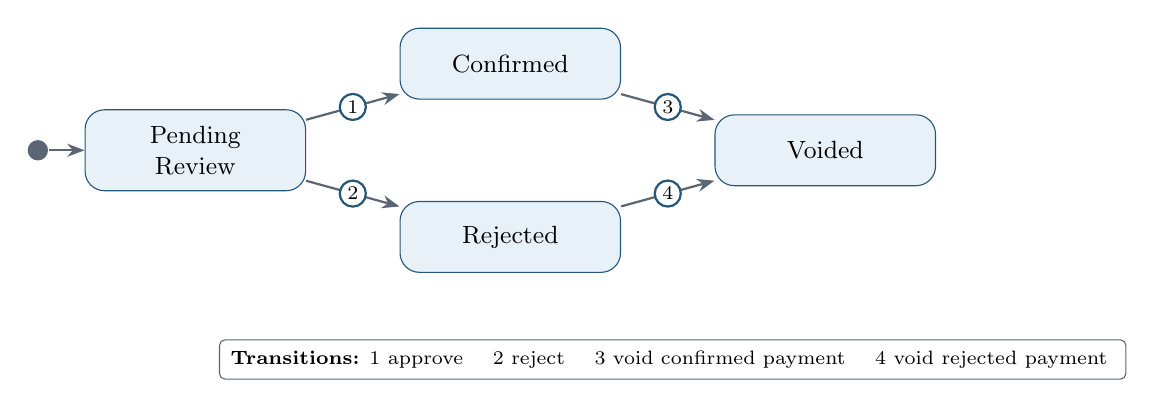
\begin{tikzpicture}[font=\small]
  \tikzset{stag/.style={circle, draw=primary, fill=white, inner sep=1.2pt, font=\scriptsize}}
  \node[circle, fill=linegray, inner sep=2.6pt] (init) at (-1,1.4) {};
  \node[state] (pending) at (1.0,1.4) {Pending\\Review};
  \node[state] (confirmed) at (5.0,2.5) {Confirmed};
  \node[state] (rejected) at (5.0,0.3) {Rejected};
  \node[state] (voided) at (9.0,1.4) {Voided};

  \draw[arrow] (init) -- (pending);
  \draw[arrow] (pending) -- node[stag, midway] {1} (confirmed);
  \draw[arrow] (pending) -- node[stag, midway] {2} (rejected);
  \draw[arrow] (confirmed) -- node[stag, midway] {3} (voided);
  \draw[arrow] (rejected) -- node[stag, midway] {4} (voided);

  \node[draw=linegray, fill=white, rounded corners=2pt, align=left, inner sep=4pt, anchor=north west, font=\scriptsize] at (1.3,-1.0) {
    \textbf{Transitions:}
    1 approve \quad 2 reject \quad 3 void confirmed payment \quad 4 void rejected payment
  };
\end{tikzpicture}%
}
\caption{State diagram for a payment submission}
\end{figure}

\subsection{Domain Model}
The domain model shows the main conceptual objects before implementation-specific fields are introduced in the database design. It highlights three central relationships: students have assignments over time, assignments bind students to beds, and invoices are settled through reviewed payments.

\begin{figure}[H]
\centering
\resizebox{\textwidth}{!}{%
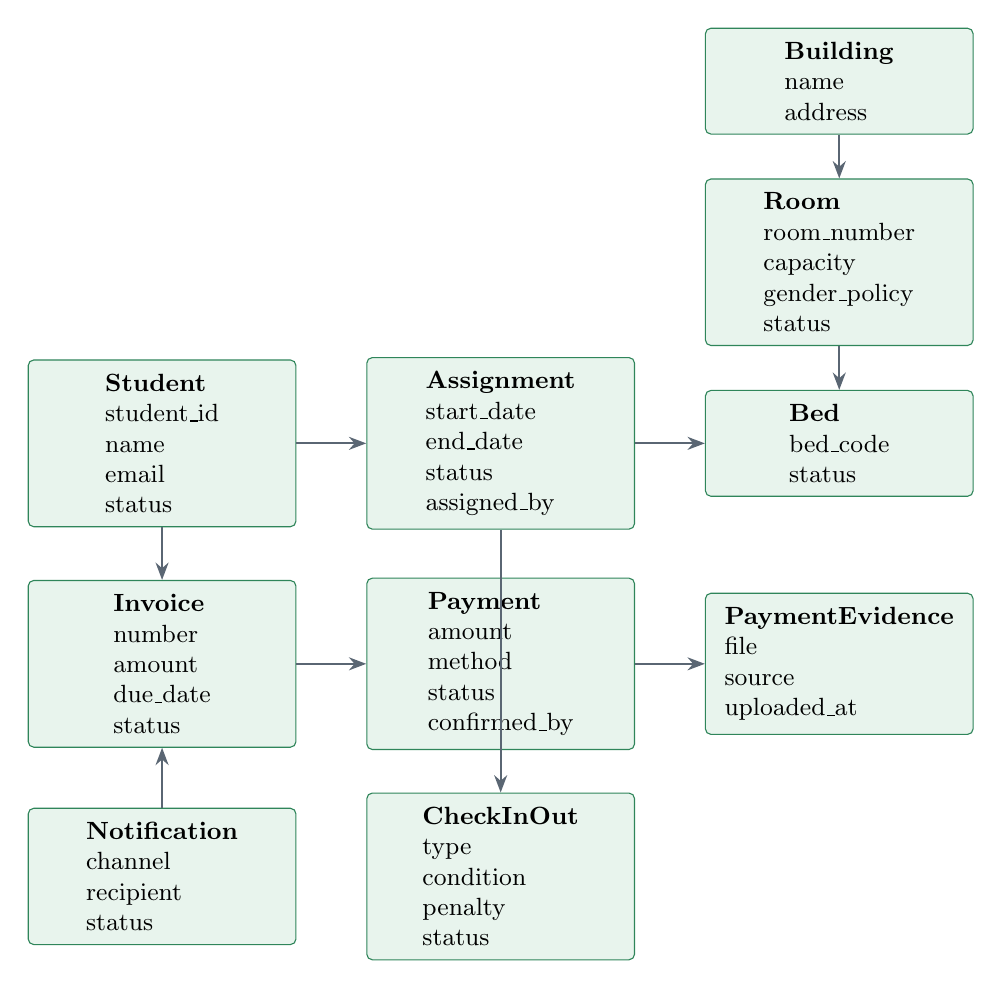
\begin{tikzpicture}[font=\small]
  \node[entity] (student) at (0,0) {\textbf{Student}\\student\_id\\name\\email\\status};
  \node[entity] (assignment) at (4.3,0) {\textbf{Assignment}\\start\_date\\end\_date\\status\\assigned\_by};
  \node[entity] (bed) at (8.6,0) {\textbf{Bed}\\bed\_code\\status};
  \node[entity] (room) at (8.6,2.3) {\textbf{Room}\\room\_number\\capacity\\gender\_policy\\status};
  \node[entity] (building) at (8.6,4.6) {\textbf{Building}\\name\\address};

  \node[entity] (invoice) at (0,-2.8) {\textbf{Invoice}\\number\\amount\\due\_date\\status};
  \node[entity] (payment) at (4.3,-2.8) {\textbf{Payment}\\amount\\method\\status\\confirmed\_by};
  \node[entity] (evidence) at (8.6,-2.8) {\textbf{PaymentEvidence}\\file\\source\\uploaded\_at};

  \node[entity] (checkin) at (4.3,-5.5) {\textbf{CheckInOut}\\type\\condition\\penalty\\status};
  \node[entity] (notice) at (0,-5.5) {\textbf{Notification}\\channel\\recipient\\status};

  \draw[arrow] (student) -- (assignment);
  \draw[arrow] (assignment) -- (bed);
  \draw[arrow] (building) -- (room);
  \draw[arrow] (room) -- (bed);
  \draw[arrow] (student) -- (invoice);
  \draw[arrow] (invoice) -- (payment);
  \draw[arrow] (payment) -- (evidence);
  \draw[arrow] (assignment) -- (checkin);
  \draw[arrow] (notice) -- (invoice);
\end{tikzpicture}%
}
\caption{Domain model}
\end{figure}

The domain model deliberately omits database implementation details such as foreign-key column names. Those details are added in Section 7. The purpose here is to define the stable vocabulary used by requirements, services, tests, and user-interface labels.

\subsection{Data Flow Diagram}
The Level 0 DFD identifies processes, data stores, external entities, and major information flows. It complements the use case model by showing where records are created or consumed. The numbered legend keeps flow names readable while still making the data movement explicit.

\begin{figure}[H]
\centering
\resizebox{\textwidth}{!}{%
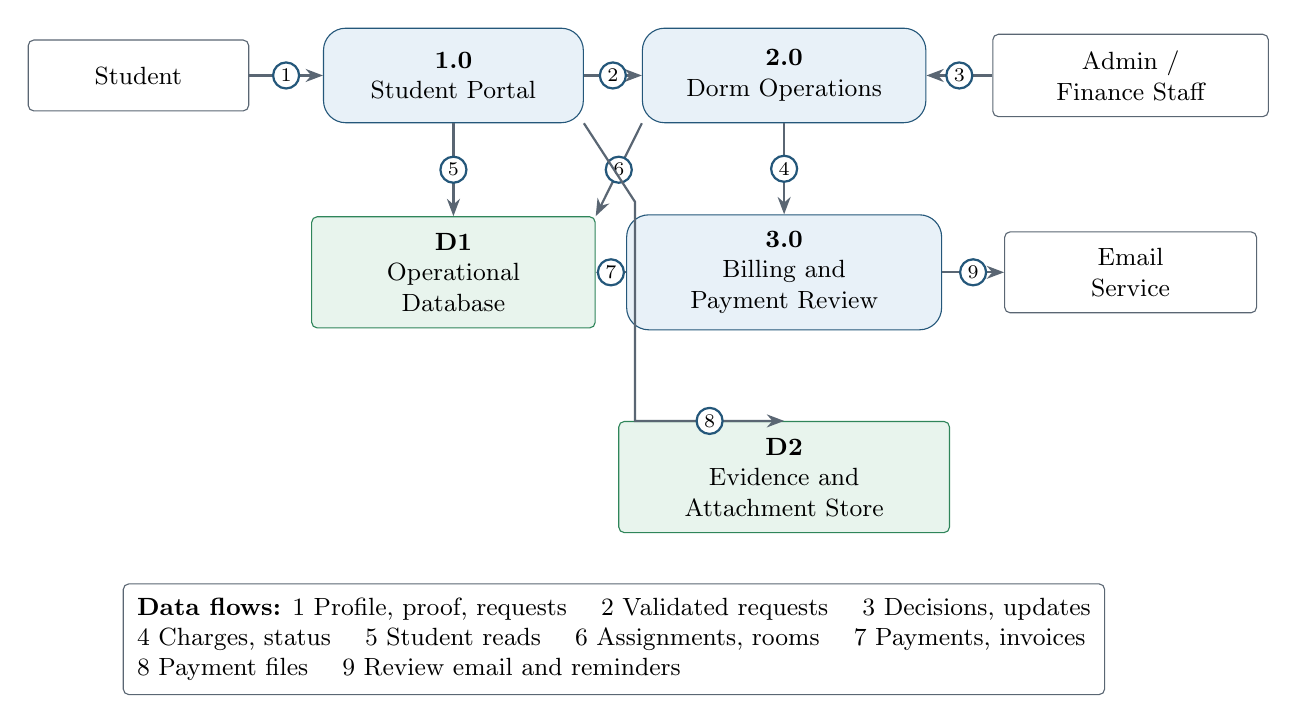
\begin{tikzpicture}[font=\small]
  \node[external, minimum width=28mm] (student) at (0,3.0) {Student};
  \node[process, minimum width=33mm] (portal) at (4.0,3.0) {\textbf{1.0}\\Student Portal};
  \node[process, minimum width=36mm] (ops) at (8.2,3.0) {\textbf{2.0}\\Dorm Operations};
  \node[external, minimum width=35mm] (staff) at (12.6,3.0) {Admin /\\Finance Staff};

  \node[data, minimum width=36mm] (db) at (4.0,0.5) {\textbf{D1}\\Operational\\Database};
  \node[process, minimum width=40mm] (billing) at (8.2,0.5) {\textbf{3.0}\\Billing and\\Payment Review};
  \node[external, minimum width=32mm] (email) at (12.6,0.5) {Email\\Service};
  \node[data, minimum width=42mm] (files) at (8.2,-2.1) {\textbf{D2}\\Evidence and\\Attachment Store};

  \tikzset{flowtag/.style={circle, draw=primary, fill=white, inner sep=1.2pt, font=\scriptsize}}

  \draw[arrow] (student) -- node[flowtag, midway] {1} (portal);
  \draw[arrow] (portal) -- node[flowtag, midway] {2} (ops);
  \draw[arrow] (staff) -- node[flowtag, midway] {3} (ops);
  \draw[arrow] (ops) -- node[flowtag, midway] {4} (billing);
  \draw[arrow] (portal) -- node[flowtag, midway] {5} (db);
  \draw[arrow] (ops.south west) -- node[flowtag, midway] {6} (db.north east);
  \draw[arrow] (billing.west) -- node[flowtag, midway] {7} (db.east);
  \draw[arrow] (portal.south east) -- ++(0.65,-1.0) coordinate (proofroute) -- (proofroute |- files.north) -- node[flowtag, midway] {8} (files.north);
  \draw[arrow] (billing) -- node[flowtag, midway] {9} (email);

  \node[draw=linegray, align=left, fill=white, rounded corners=2pt, inner sep=5pt, anchor=north west] at (-0.2,-3.45) {
    \textbf{Data flows:}
    1 Profile, proof, requests \quad
    2 Validated requests \quad
    3 Decisions, updates\\
    4 Charges, status \quad
    5 Student reads \quad
    6 Assignments, rooms \quad
    7 Payments, invoices\\
    8 Payment files \quad
    9 Review email and reminders
  };
\end{tikzpicture}%
}
\caption{Level 0 data flow diagram}
\end{figure}

\section{System Design Overview}

\subsection{Design Approach}
The design transforms the analysis model into a modular Django application. Each operational area is implemented as a Django app with models, forms, views, templates, service classes, permissions, and tests. Business rules that affect correctness, such as bed assignment, payment confirmation, invoice settlement, and check-out release, are implemented in service classes instead of being embedded directly in views.

The selected implementation style is a server-rendered Django application rather than a split React front end and separate API backend. A split design would be useful for a large multi-client product, but it would add a separate build pipeline, cross-origin configuration, duplicated form validation, and more deployment moving parts for this course MVP. Django templates, forms, Bootstrap, and HTMX are sufficient for the planned demo while still allowing REST-style JSON endpoints under \texttt{/api/v1} for asynchronous widgets and future integrations.

\subsection{MVP Subsystems}

\begin{longtable}{L{0.22\textwidth} L{0.44\textwidth} L{0.22\textwidth}}
\toprule
\textbf{Subsystem} & \textbf{Responsibilities} & \textbf{Primary Users}\\
\midrule
\endhead
Identity and Access & Authentication, role mapping, permission checks, user profile linkage. & All users\\
Resident Management & Student profiles, resident status, contacts, search, import, history. & Admin, Student\\
Room Inventory & Buildings, floors, rooms, beds, capacity, bed state transitions. & Admin\\
Assignment and Occupancy & Assignment recommendation, reservation, check-in activation, transfer, release. & Admin\\
Billing & Invoice generation, line items, deposits, rent, fees, penalties, outstanding balance. & Finance\\
Payment Review & Evidence upload, pending payment queue, email summary, confirmation, rejection. & Student, Finance\\
Communication & Announcements, reminders, notification log. & Admin, Finance, Student\\
Reporting & Occupancy dashboard, finance dashboard, downloadable summaries. & Admin, Finance, Management\\
Demo Data & Synthetic student, room, invoice, payment, and assignment data generation. & Developers, Demo users\\
\bottomrule
\end{longtable}

\subsection{Planned Django App Layout}
The implementation should be organised as a layered Django project. Each app owns its models, forms, views, templates, services, permissions, and tests. Shared helpers are kept small and framework-aware code should not leak into domain services.

\begin{verbatim}
dorm_system/
  config/                 # settings, urls, ASGI/WSGI
  accounts/               # auth extensions, roles, permissions
  residents/              # student profiles and resident history
  rooms/                  # building, floor, room, bed inventory
  assignments/            # recommendation, reservation, transfer, check-in
  billing/                # invoices, invoice lines, balances, overdue rules
  payments/               # payment evidence upload and finance review
  communications/         # announcements, reminders, notification log
  reports/                # dashboards, CSV exports, aggregate queries
  demo_data/              # seed command and synthetic fixtures
  common/                 # audit log, status helpers, file validators
\end{verbatim}

The main dependency direction is:
\begin{center}
\texttt{templates/forms/views -> services -> models/querysets -> database}
\end{center}
Views may import services and forms. Services may import models, querysets, gateways, and audit helpers. Models must not import views or templates. This rule keeps the layered design testable.

\subsection{High-Level Request Flow}
\begin{enumerate}
  \item Browser sends a request to a Django view.
  \item Middleware authenticates the user session and applies security controls.
  \item The view validates permissions and form or JSON input.
  \item The view calls a service class for business logic.
  \item The service reads and writes models inside a transaction where consistency matters.
  \item The result is returned as an HTML page, HTMX partial, redirect, or JSON response.
  \item Notification tasks send email after database changes are committed.
\end{enumerate}

\section{Architectural Design}

\subsection{Architecture Style}
The system uses a layered MVC-style client-server architecture implemented as a modular Django monolith. The browser receives HTML for primary pages, while selected JSON endpoints provide stable contracts for dashboard widgets, recommendations, and future clients. This keeps the local demo simple without removing a later path to a separate front end.

\begin{itemize}
  \item \textbf{Presentation layer}: Django templates, Bootstrap components, and HTMX partial updates.
  \item \textbf{Controller layer}: Django views and URL routes.
  \item \textbf{Application service layer}: assignment, billing, payment, notification, and reporting services.
  \item \textbf{Domain/data layer}: Django models, querysets, constraints, and PostgreSQL.
  \item \textbf{Integration layer}: email service, file storage, import/export, and future external systems.
\end{itemize}

\subsection{Design Goals and Principles}
The design follows the same analysis-to-design discipline used in the reference report: every design principle is tied to a concrete implementation mechanism. The main goal is a layered monolith that is simple enough for a project demo but structured enough to extend after the MVP.

\begin{longtable}{L{0.20\textwidth} L{0.34\textwidth} L{0.33\textwidth}}
\toprule
\textbf{Principle} & \textbf{Meaning in This System} & \textbf{Implementation Mechanism}\\
\midrule
\endhead
Abstraction & Controllers should not know the details of assignment scoring, invoice settlement, file storage, or email delivery. & Service classes expose intention-revealing methods such as \texttt{reserve\_bed}, \texttt{confirm\_payment}, and \texttt{send\_digest}.\\
Modularity & Each business capability should have one main place to change. & Separate Django apps for accounts, residents, rooms, assignments, billing, payments, notifications, reports, and demo data.\\
High cohesion & A module should own one operational responsibility. & Assignment logic stays in the assignment service; invoice balance logic stays in billing; payment evidence review stays in payments.\\
Low coupling & Modules should interact through stable calls rather than shared implementation details. & Views call services; services use model/query APIs and integration gateways; templates do not perform business decisions.\\
Information hiding & Volatile external decisions should be isolated. & Email, file storage, future payment gateways, and future university SSO are hidden behind small gateway functions.\\
\bottomrule
\end{longtable}

\subsection{Design Patterns Applied}
The system deliberately uses a small set of patterns that fit a Django MVP. These patterns are selected because they make the implementation easier to reason about rather than because the project needs heavyweight architecture.

\begin{longtable}{L{0.19\textwidth} L{0.30\textwidth} L{0.38\textwidth}}
\toprule
\textbf{Pattern} & \textbf{Problem Solved} & \textbf{Use and Benefit in This System}\\
\midrule
\endhead
Layered MVC / Django MTV & Page rendering, request handling, workflow rules, and persistence can become mixed together. & Templates render pages, views validate requests and permissions, services coordinate workflows, and models persist state. This keeps each layer understandable during implementation.\\
Service Layer & Assignment, checkout, billing, and payment review require multi-step rules and transactions. & Assignment, billing, payment, checkout, and notification services keep workflow rules out of views and templates.\\
Strategy & Assignment scoring may change after the MVP. & \texttt{AssignmentScorer} starts with a policy-based scorer; preference-based or roommate-matching scorers can be added later without rewriting the assignment service.\\
State & Beds, assignments, invoices, payments, and notifications have legal lifecycle transitions. & Status fields and service validators prevent invalid transitions such as confirming a rejected payment or occupying a maintenance bed.\\
Repository / Query Object & Dashboard and queue screens need repeated filtered queries. & Django managers/querysets provide named methods such as \texttt{available\_beds()}, \texttt{pending\_payments()}, and \texttt{overdue\_invoices()}, improving reuse and testability.\\
Adapter / Gateway & Email, file storage, SSO, and payment providers may differ between demo and deployment. & \texttt{EmailGateway} and \texttt{FileStorageGateway} isolate provider details so services do not depend on local disk or one SMTP implementation.\\
Observer & Follow-up work should happen after important events without cluttering core workflows. & Payment upload, invoice overdue marking, and announcement publishing create notification events consumed by the notification service.\\
\bottomrule
\end{longtable}

\subsection{Architecture Diagram}
The architecture diagram gives the high-level dependency rule: browser interactions enter through Django views, views call services, services coordinate domain models and gateways, and persistent state is stored in PostgreSQL or media storage. Dependencies point downward; templates and views must not contain assignment, billing, or payment-review rules.

\begin{figure}[H]
\centering
\resizebox{\textwidth}{!}{%
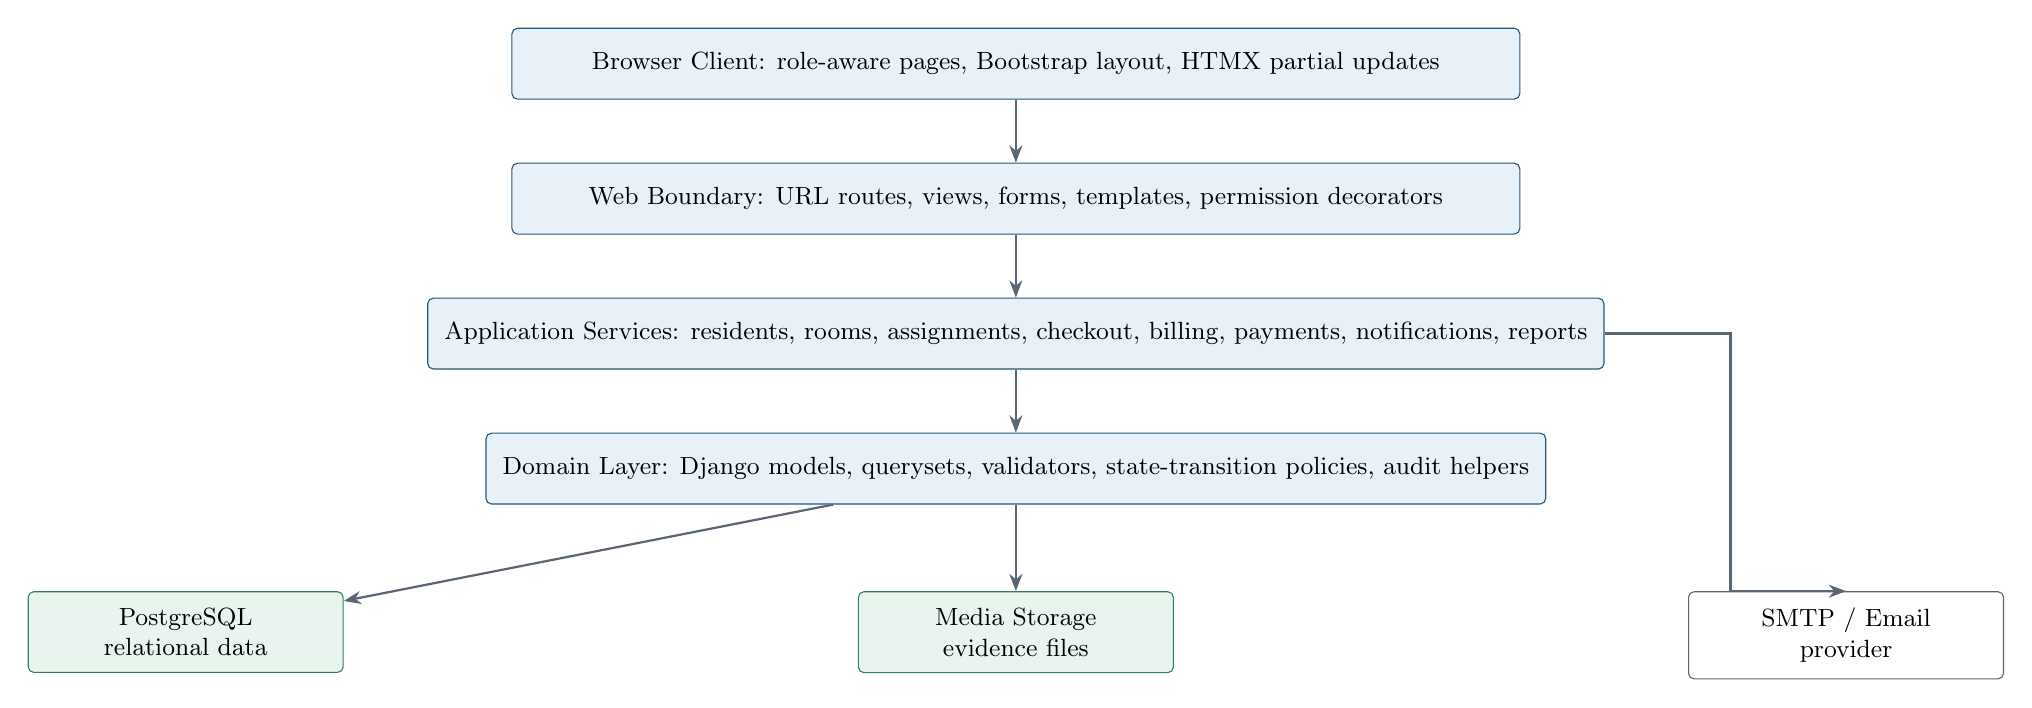
\begin{tikzpicture}[node distance=8mm, font=\small]
  \node[module, minimum width=128mm] (client) {Browser Client: role-aware pages, Bootstrap layout, HTMX partial updates};
  \node[module, below=of client, minimum width=128mm] (web) {Web Boundary: URL routes, views, forms, templates, permission decorators};
  \node[module, below=of web, minimum width=128mm] (services) {Application Services: residents, rooms, assignments, checkout, billing, payments, notifications, reports};
  \node[module, below=of services, minimum width=128mm] (domain) {Domain Layer: Django models, querysets, validators, state-transition policies, audit helpers};
  \node[data, below left=11mm and 18mm of domain, minimum width=40mm] (db) {PostgreSQL\\relational data};
  \node[data, below=11mm of domain, minimum width=40mm] (files) {Media Storage\\evidence files};
  \node[external, below right=11mm and 18mm of domain, minimum width=40mm] (email) {SMTP / Email\\provider};

  \draw[arrow] (client) -- (web);
  \draw[arrow] (web) -- (services);
  \draw[arrow] (services) -- (domain);
  \draw[arrow] (domain) -- (db);
  \draw[arrow] (domain) -- (files);
  \draw[arrow] (services.east) -- ++(16mm,0) |- (email.north);
\end{tikzpicture}%
}
\caption{Layered MVC architecture}
\end{figure}

\subsection{Package and Layer Decomposition}
The package view turns the architecture into an implementation map. Each package corresponds to a Django app or a small shared support package. The presentation and controller packages depend on service packages; service packages depend on domain packages and infrastructure gateways. This decomposition is the main maintainability mechanism because a future payment gateway, SSO adapter, or visitor module can be added at a clear package boundary.

\begin{figure}[H]
\centering
\resizebox{\textwidth}{!}{%
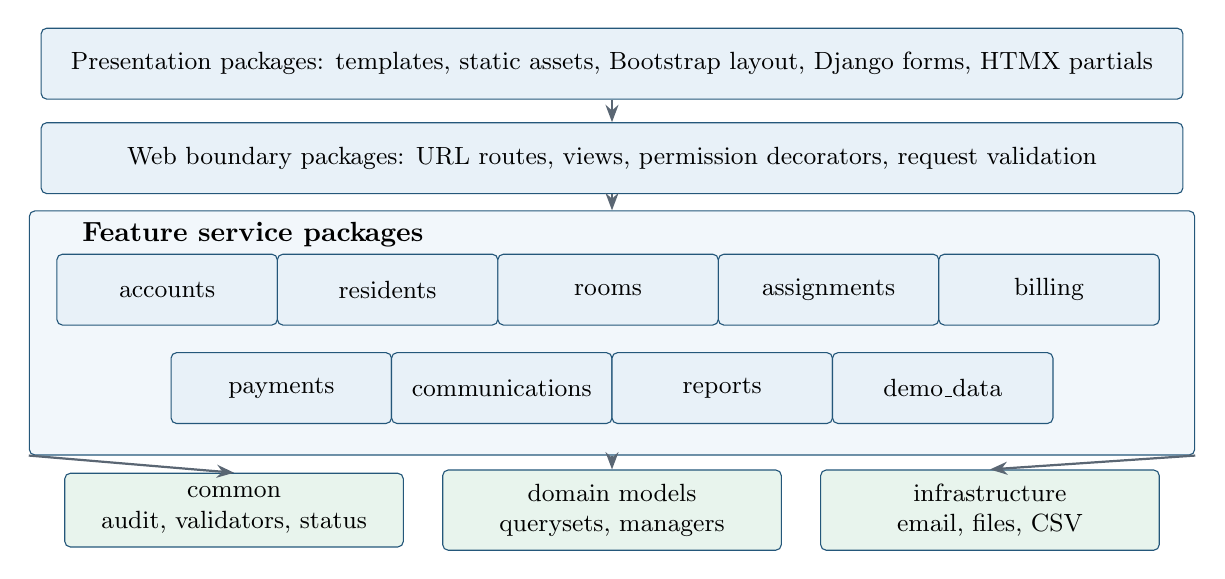
\begin{tikzpicture}[font=\scriptsize]
  \node[packagebox, minimum width=145mm] (presentation) at (0,5.2)
    {Presentation packages: templates, static assets, Bootstrap layout, Django forms, HTMX partials};
  \node[packagebox, minimum width=145mm] (boundary) at (0,4.0)
    {Web boundary packages: URL routes, views, permission decorators, request validation};

  \node[draw=primary, rounded corners=2pt, fill=softblue!55, minimum width=148mm, minimum height=31mm] (featurebox) at (0,1.78) {};
  \node[anchor=west, font=\bfseries] at (-6.85,3.03) {Feature service packages};
  \node[packagebox, minimum width=28mm] at (-5.65,2.33) {accounts};
  \node[packagebox, minimum width=28mm] at (-2.85,2.33) {residents};
  \node[packagebox, minimum width=28mm] at (-0.05,2.33) {rooms};
  \node[packagebox, minimum width=28mm] at (2.75,2.33) {assignments};
  \node[packagebox, minimum width=28mm] at (5.55,2.33) {billing};
  \node[packagebox, minimum width=28mm] at (-4.2,1.08) {payments};
  \node[packagebox, minimum width=28mm] at (-1.4,1.08) {communications};
  \node[packagebox, minimum width=28mm] at (1.4,1.08) {reports};
  \node[packagebox, minimum width=28mm] at (4.2,1.08) {demo\_data};

  \node[packagebox, minimum width=43mm, fill=softgreen] (common) at (-4.8,-0.47)
    {common\\audit, validators, status};
  \node[packagebox, minimum width=43mm, fill=softgreen] (models) at (0,-0.47)
    {domain models\\querysets, managers};
  \node[packagebox, minimum width=43mm, fill=softgreen] (infra) at (4.8,-0.47)
    {infrastructure\\email, files, CSV};

  \draw[arrow] (presentation) -- (boundary);
  \draw[arrow] (boundary) -- (featurebox.north);
  \draw[arrow] (featurebox.south west) -- (common.north);
  \draw[arrow] (featurebox.south) -- (models.north);
  \draw[arrow] (featurebox.south east) -- (infra.north);
\end{tikzpicture}%
}
\caption{Package and layer decomposition}
\end{figure}

\subsection{Component Diagram}
The component diagram opens the server box and shows deployable or replaceable components. The important design point is that external systems are reached through gateway components. For example, \texttt{PaymentReviewService} does not know whether files are local or S3-compatible; it only calls the file-storage gateway.

\begin{figure}[H]
\centering
\resizebox{\textwidth}{!}{%
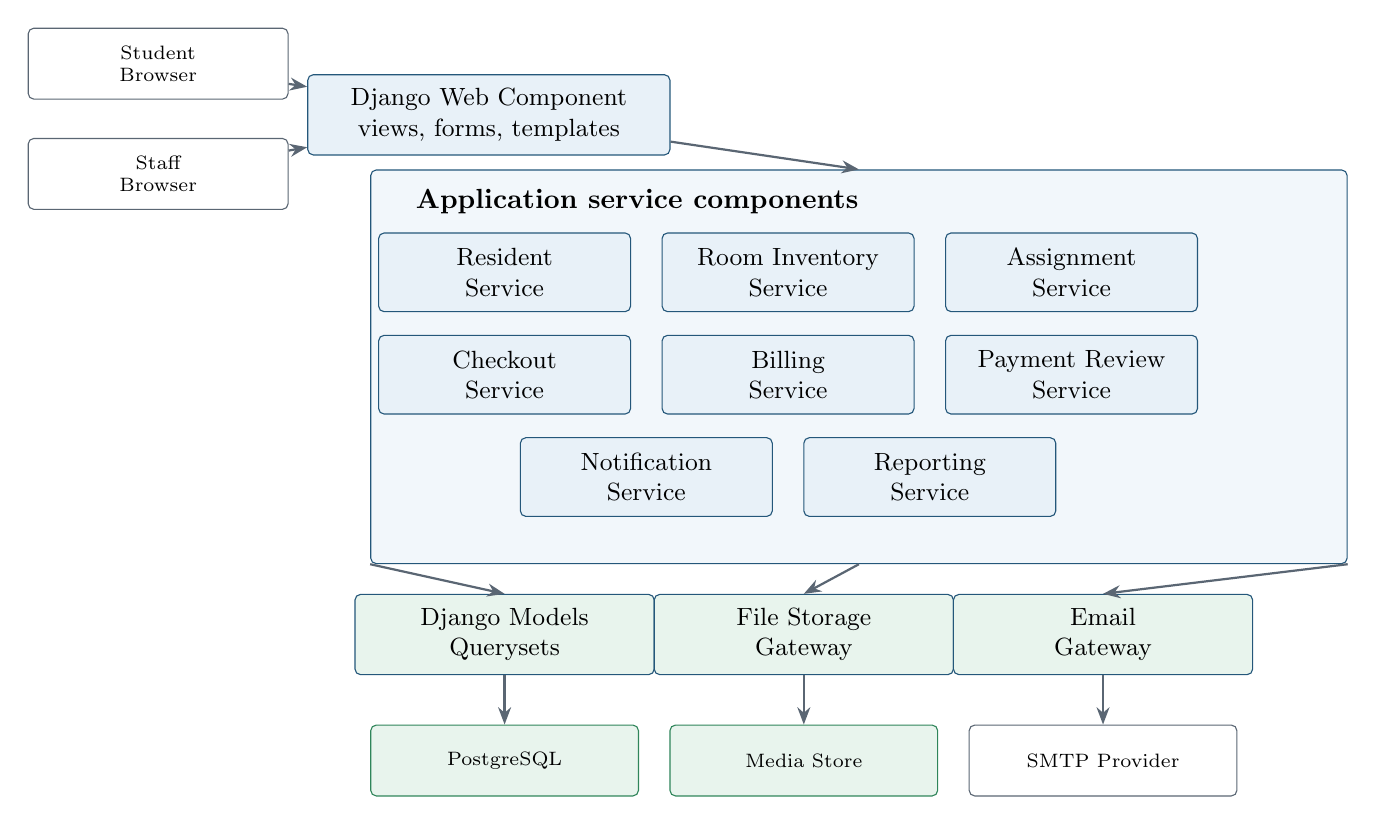
\begin{tikzpicture}[font=\scriptsize]
  \node[external, minimum width=33mm] (student) at (-5.2,5.0) {Student\\Browser};
  \node[external, minimum width=33mm] (staff) at (-5.2,3.6) {Staff\\Browser};
  \node[componentbox, minimum width=46mm] (web) at (-1.0,4.35) {Django Web Component\\views, forms, templates};

  \node[draw=primary, rounded corners=2pt, fill=softblue!55, minimum width=124mm, minimum height=50mm] (servicebox) at (3.7,1.15) {};
  \node[anchor=west, font=\bfseries] at (-2.05,3.25) {Application service components};
  \node[componentbox, minimum width=32mm] at (-0.8,2.35) {Resident\\Service};
  \node[componentbox, minimum width=32mm] at (2.8,2.35) {Room Inventory\\Service};
  \node[componentbox, minimum width=32mm] at (6.4,2.35) {Assignment\\Service};
  \node[componentbox, minimum width=32mm] at (-0.8,1.05) {Checkout\\Service};
  \node[componentbox, minimum width=32mm] at (2.8,1.05) {Billing\\Service};
  \node[componentbox, minimum width=32mm] at (6.4,1.05) {Payment Review\\Service};
  \node[componentbox, minimum width=32mm] at (1.0,-0.25) {Notification\\Service};
  \node[componentbox, minimum width=32mm] at (4.6,-0.25) {Reporting\\Service};

  \node[componentbox, minimum width=38mm, fill=softgreen] (models) at (-0.8,-2.25) {Django Models\\Querysets};
  \node[componentbox, minimum width=38mm, fill=softgreen] (files) at (3.0,-2.25) {File Storage\\Gateway};
  \node[componentbox, minimum width=38mm, fill=softgreen] (email) at (6.8,-2.25) {Email\\Gateway};

  \node[data, minimum width=34mm] (db) at (-0.8,-3.85) {PostgreSQL};
  \node[data, minimum width=34mm] (media) at (3.0,-3.85) {Media Store};
  \node[external, minimum width=34mm] (smtp) at (6.8,-3.85) {SMTP Provider};

  \draw[arrow] (student) -- (web);
  \draw[arrow] (staff) -- (web);
  \draw[arrow] (web) -- (servicebox.north);
  \draw[arrow] (servicebox.south west) -- (models.north);
  \draw[arrow] (servicebox.south) -- (files.north);
  \draw[arrow] (servicebox.south east) -- (email.north);
  \draw[arrow] (models) -- (db);
  \draw[arrow] (files) -- (media);
  \draw[arrow] (email) -- (smtp);
\end{tikzpicture}%
}
\caption{Component diagram}
\end{figure}

\subsection{Technology Stack}

\begin{longtable}{L{0.22\textwidth} L{0.25\textwidth} L{0.40\textwidth}}
\toprule
\textbf{Layer} & \textbf{Selected Technology} & \textbf{Rationale}\\
\midrule
\endhead
Frontend & Django templates, Bootstrap, HTMX & Fast MVP development, responsive interface, server-rendered pages, simple partial updates.\\
Backend & Python, Django & Mature web framework with ORM, authentication, admin tools, forms, migrations, and testing support.\\
API & Django JSON views, optional Django REST Framework later & Keeps MVP dependencies small while preserving versioned REST contracts for integrations.\\
Database & PostgreSQL & Strong relational integrity, transactions, constraints, indexes, and reporting support.\\
Authentication & Django auth with role groups & Suitable for MVP role-based access. Can later integrate OAuth or university SSO.\\
Files & Local media storage for demo, S3-compatible storage for deployment & Stores payment evidence and inspection attachments.\\
Email & SMTP or console backend in development & Supports reminders and payment review summaries.\\
Deployment & Docker Compose or cloud VM/container & Repeatable local demo and simple production migration path.\\
\bottomrule
\end{longtable}

This stack is intentionally conservative. Express or FastAPI with React would provide clearer separation for a public API product, but it would require more boilerplate, more testing surfaces, and an additional Node-based front-end build. For the project schedule, Django provides authentication, validation, forms, database migrations, admin utilities, and server-rendered pages in one deployable unit. The architecture still leaves an upgrade path: if a React or mobile client is added later, the \texttt{/api/v1} endpoints and service layer can become the stable backend contract.

\subsection{Deployment Overview}
For the demo, the system can run on one development machine using Docker Compose. The browser connects to a reverse proxy or directly to Django in development. The Django container talks to PostgreSQL, writes media files to a persistent volume, and sends email through either the console backend or an SMTP provider. This topology is practical for a local presentation because it avoids a separate frontend server and can be reset with migrations plus synthetic seed data. The same topology can move to a low-cost VM or container host by replacing the local media volume with S3-compatible storage, adding managed PostgreSQL if needed, and terminating TLS at the reverse proxy.

\begin{figure}[H]
\centering
\resizebox{\textwidth}{!}{%
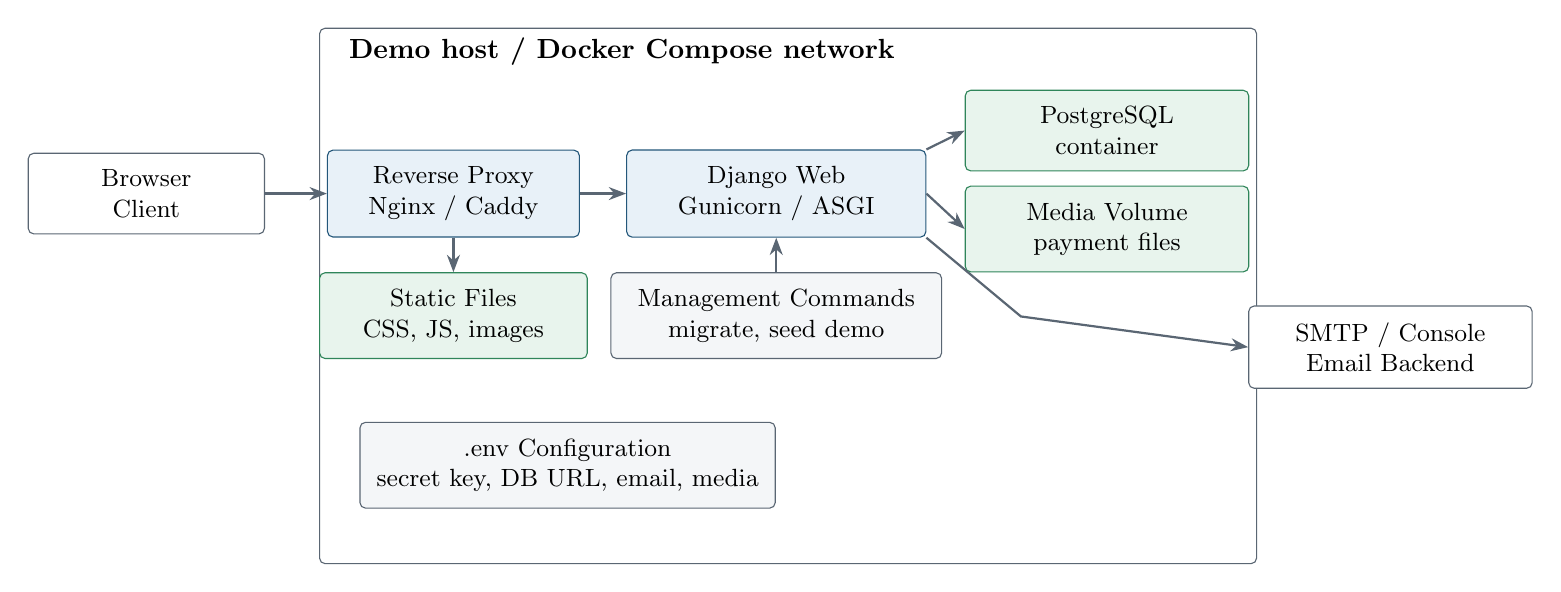
\begin{tikzpicture}[font=\small]
  \node[external, minimum width=30mm] (browser) at (-0.2,2.7) {Browser\\Client};
  \draw[draw=linegray, rounded corners=2pt] (2.0,-2.0) rectangle (13.9,4.8);
  \node[anchor=west, font=\bfseries] at (2.25,4.5) {Demo host / Docker Compose network};

  \node[module, minimum width=32mm] (proxy) at (3.7,2.7) {Reverse Proxy\\Nginx / Caddy};
  \node[module, minimum width=38mm] (web) at (7.8,2.7) {Django Web\\Gunicorn / ASGI};
  \node[data, minimum width=34mm] (static) at (3.7,1.15) {Static Files\\CSS, JS, images};
  \node[box, minimum width=42mm] (cmd) at (7.8,1.15) {Management Commands\\migrate, seed demo};
  \node[data, minimum width=36mm] (db) at (12.0,3.5) {PostgreSQL\\container};
  \node[data, minimum width=36mm] (media) at (12.0,2.25) {Media Volume\\payment files};
  \node[box, minimum width=42mm] (env) at (5.15,-0.75) {.env Configuration\\secret key, DB URL, email, media};
  \node[external, minimum width=36mm] (smtp) at (15.6,0.75) {SMTP / Console\\Email Backend};

  \draw[arrow] (browser) -- (proxy);
  \draw[arrow] (proxy) -- (web);
  \draw[arrow] (web.north east) -- (db.west);
  \draw[arrow] (web.east) -- (media.west);
  \draw[arrow] (proxy.south) -- (static.north);
  \draw[arrow] (cmd.north) -- (web.south);
  \draw[arrow] (web.south east) -- ++(1.2,-1.0) -- (smtp.west);
\end{tikzpicture}%
}
\caption{Deployment overview}
\end{figure}

\section{Data / Class Design}

\subsection{Class Diagram}
The class design is presented as one integrated UML class diagram generated from Mermaid source. It follows the convention guide: each class has a name, private attributes, and public operations; solid lines represent associations, filled diamonds represent composition, and dashed arrows represent dependencies. Multiplicities are placed near both class ends, using values such as \texttt{1}, \texttt{0..1}, \texttt{0..*}, and \texttt{1..*}. Primary-key and foreign-key columns are intentionally reserved for the ERD and database schema sections.

\begin{figure}[H]
\centering
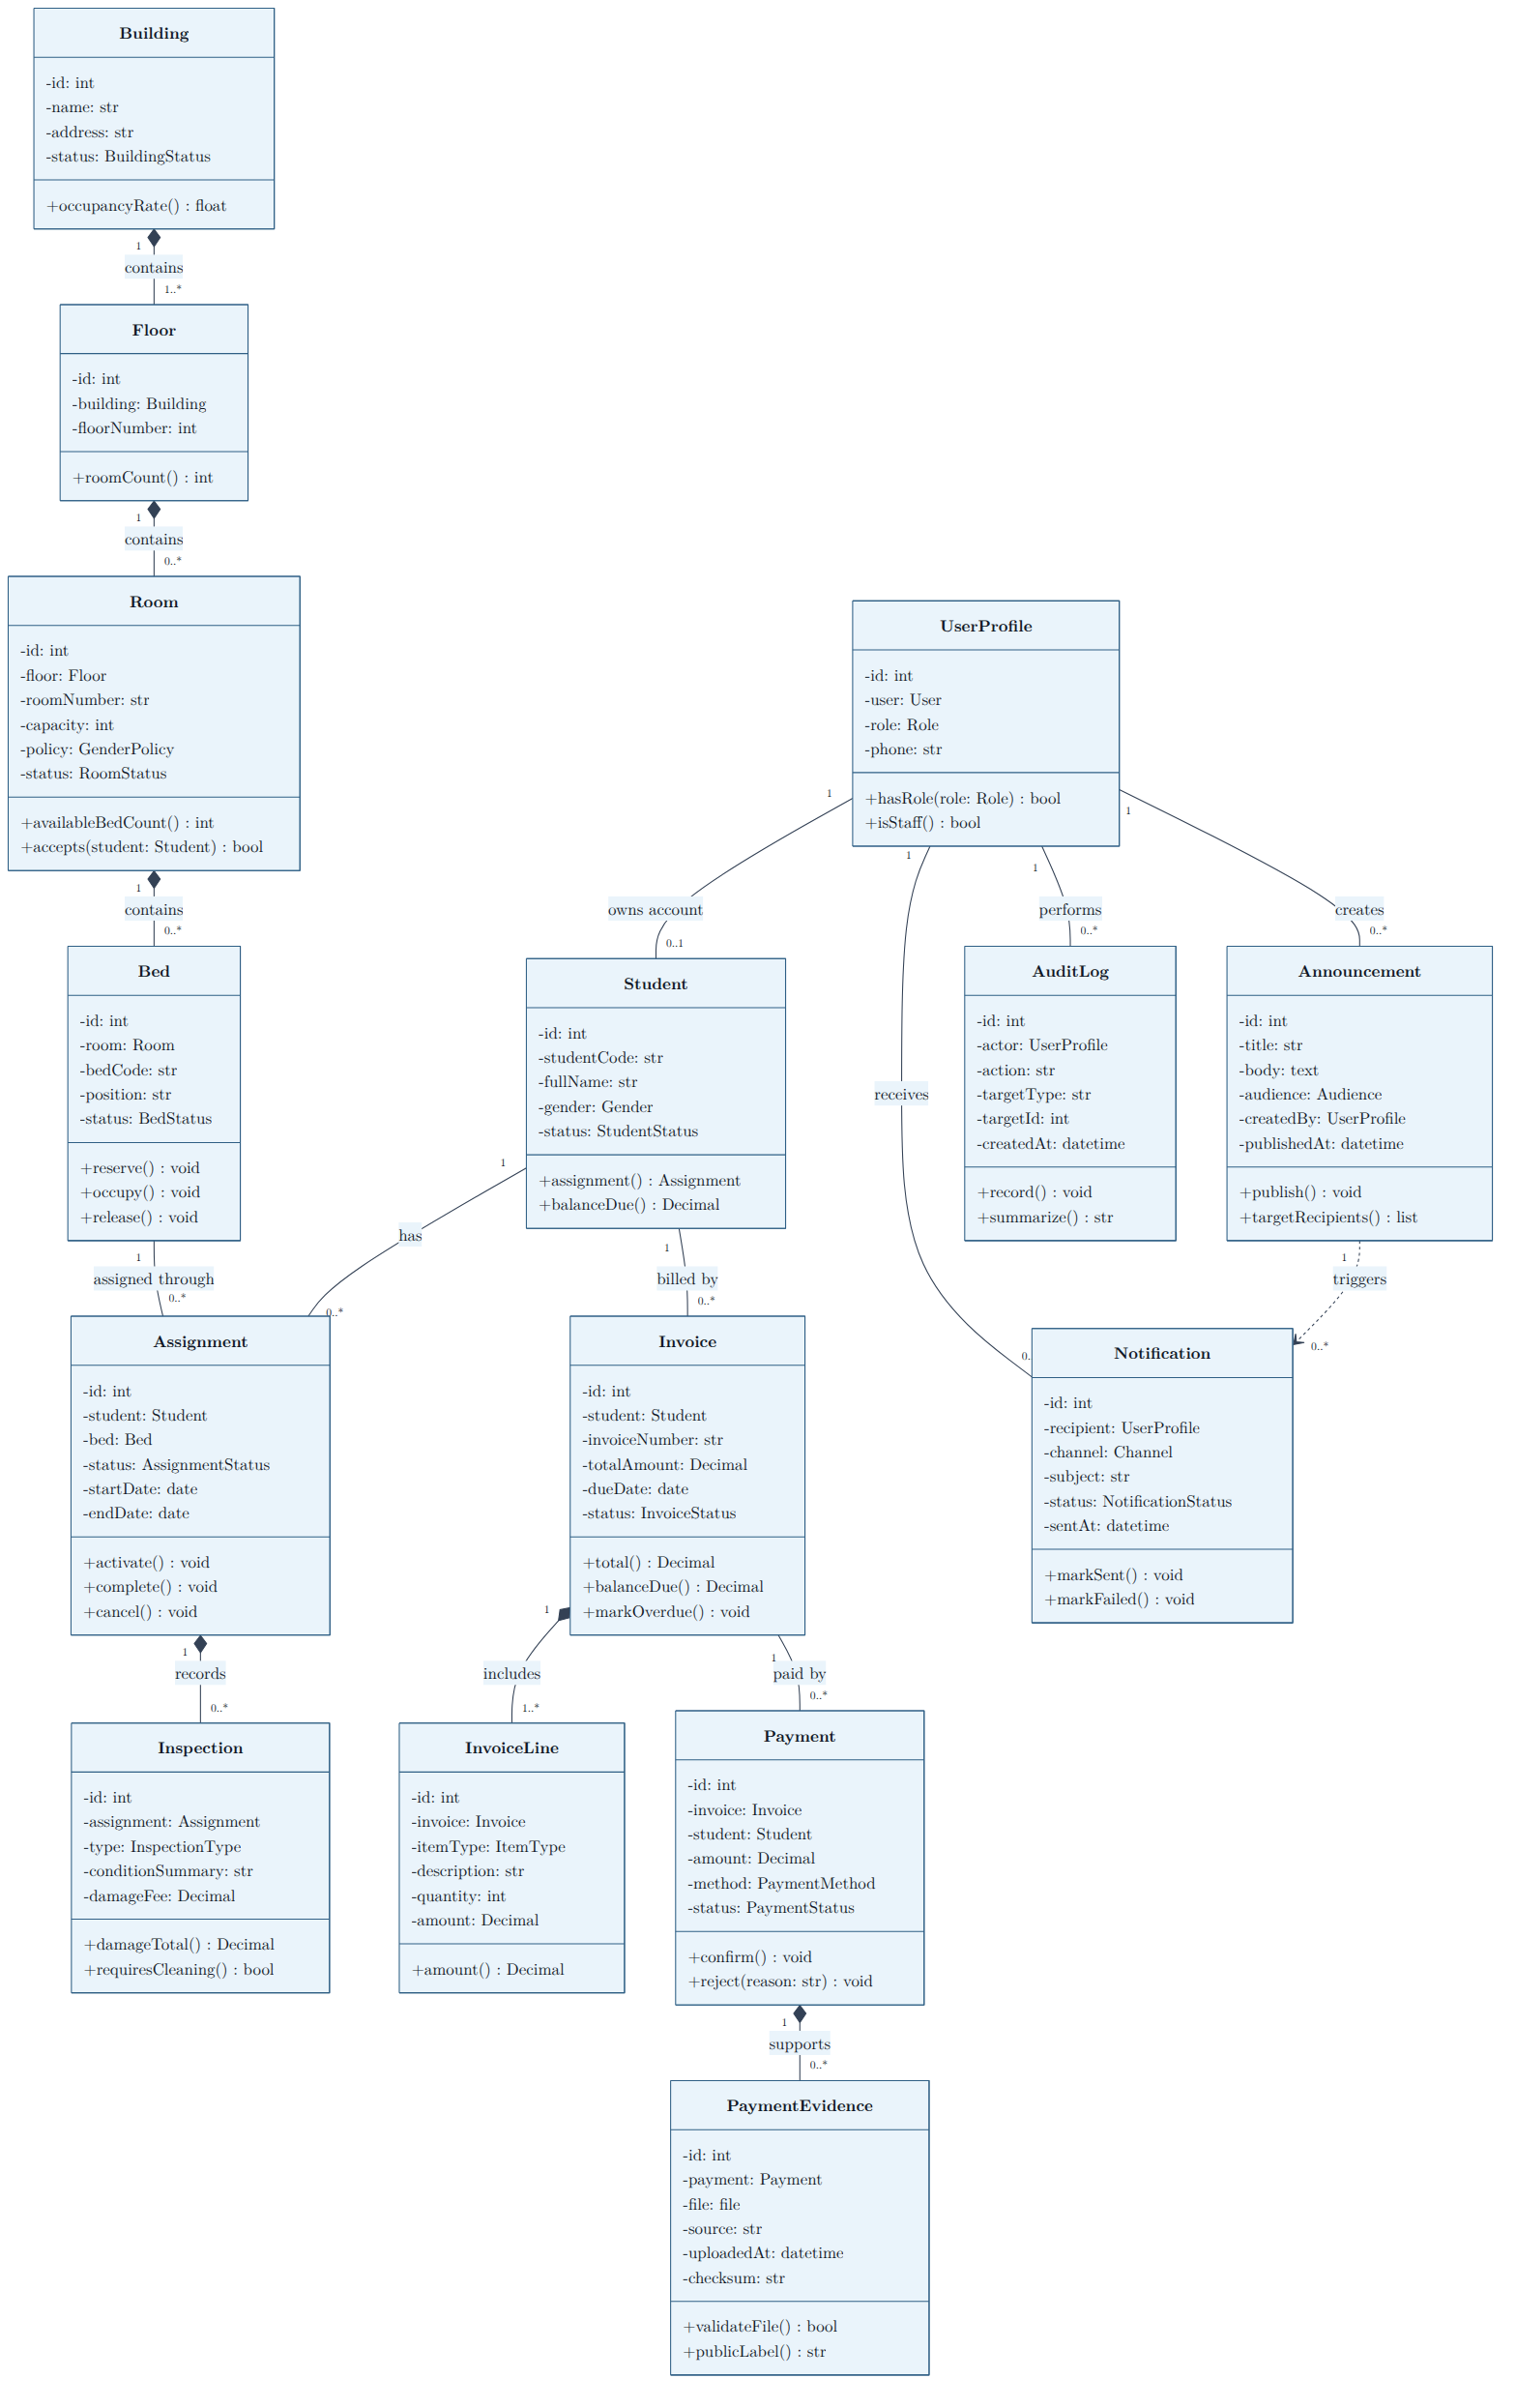
\includegraphics[width=\textwidth,height=0.86\textheight,keepaspectratio]{figures/class_diagram.png}
\caption{Unified UML class diagram for the dormitory management system}
\end{figure}

\subsection{Database Schema}

\begin{longtable}{L{0.20\textwidth} L{0.40\textwidth} L{0.27\textwidth}}
\toprule
\textbf{Table} & \textbf{Key Fields} & \textbf{Notes}\\
\midrule
\endhead
auth\_user & id, username, email, password, is\_active & Django authentication table.\\
user\_profile & id, user\_id, role, phone & Role and profile extension.\\
student & id, user\_id, student\_code, full\_name, gender, email, phone, status & Student master record.\\
building & id, name, address, status & Dorm building.\\
floor & id, building\_id, floor\_number & Optional physical grouping.\\
room & id, floor\_id, room\_number, capacity, gender\_policy, status & Room inventory and policy.\\
bed & id, room\_id, bed\_code, position, status & Assignable unit.\\
assignment & id, student\_id, bed\_id, status, start\_date, end\_date, assigned\_by\_id, reason & Occupancy history.\\
inspection & id, assignment\_id, type, condition\_summary, damage\_fee, notes, inspected\_by\_id & Check-in and check-out evidence.\\
invoice & id, student\_id, invoice\_number, total\_amount, due\_date, status & Billing header.\\
invoice\_line & id, invoice\_id, item\_type, description, quantity, unit\_price, amount & Rent, deposit, fee, penalty.\\
payment & id, invoice\_id, student\_id, amount, method, status, submitted\_at, reviewed\_by\_id & Payment review state.\\
payment\_evidence & id, payment\_id, file, source, uploaded\_at, checksum & Uploaded proof files.\\
announcement & id, title, body, audience, created\_by\_id, published\_at & Broadcast notices.\\
notification & id, recipient\_id, channel, subject, body, status, sent\_at & Email and in-app log.\\
audit\_log & id, actor\_id, action, target\_type, target\_id, old\_value, new\_value, created\_at & Audit trail.\\
\bottomrule
\end{longtable}

\subsection{Database Constraints and Indexes}
The implementation should enforce the most important business rules in the database as well as in services.

\begin{longtable}{L{0.31\textwidth} L{0.52\textwidth}}
\toprule
\textbf{Constraint / Index} & \textbf{Purpose}\\
\midrule
\endhead
Unique student code & Prevent duplicate student master records.\\
Unique room per floor & Prevent duplicate room numbers on the same floor.\\
Unique bed per room & Prevent duplicate bed codes in one room.\\
Partial unique index on active assignment per student & Enforce at most one active or reserved assignment for a student.\\
Partial unique index on active assignment per bed & Enforce at most one active or reserved assignment for a bed.\\
Unique invoice number & Keep invoice references stable for payment review.\\
Indexes on status and date fields & Support dashboards, overdue detection, and pending payment queues.\\
Foreign keys with restricted or protected delete where history matters & Preserve auditability for invoices, assignments, payments, and inspections.\\
\bottomrule
\end{longtable}

\subsection{Entity Relationships}
The ERD is presented as one generated crow-foot diagram. It keeps the database notation separate from the UML class diagram: entities are tables, attributes are database columns, PK/FK markers are shown inside the entities, and cardinality is shown on the relationship ends. Conceptually, students and beds are \textbf{N:M over time}; the implementation resolves this through the \texttt{assignment} associative entity.

\begin{figure}[H]
\centering
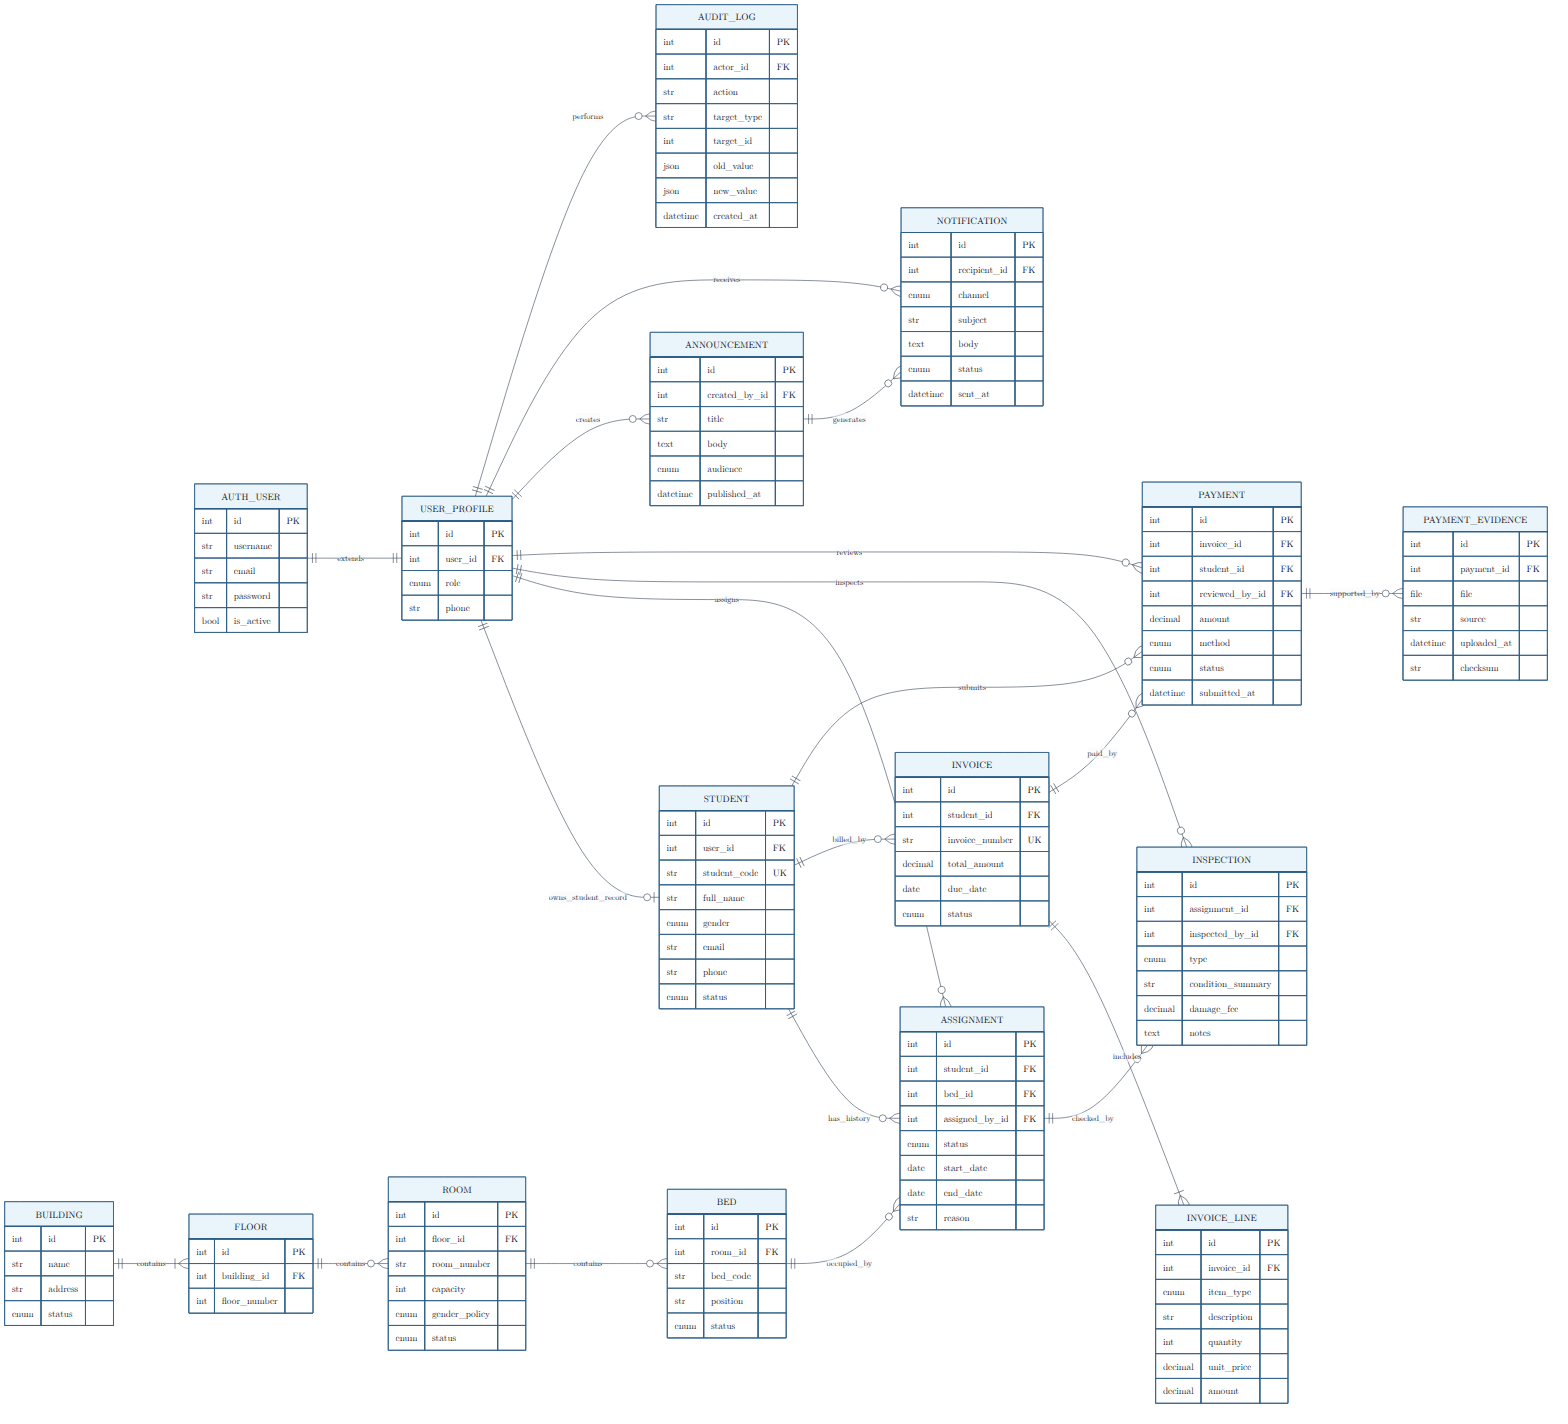
\includegraphics[width=\textwidth,height=0.78\textheight,keepaspectratio]{figures/erd_diagram.png}
\caption{Unified entity relationship diagram for the dormitory management system}
\end{figure}

The crow-foot ERD translates directly into database constraints and Django model fields. Inventory tables describe physical capacity, assignment tables describe occupancy history, billing tables describe receivables and proof review, and communication/audit tables preserve operational evidence.

\begin{longtable}{L{0.34\textwidth} L{0.18\textwidth} L{0.36\textwidth}}
\toprule
\textbf{Relationship} & \textbf{Cardinality} & \textbf{Implementation note}\\
\midrule
\endhead
UserProfile--Student & 1:0..1 & Only student accounts have a linked Student record; staff profiles do not.\\
Building--Floor & 1:1..* & A building has one or more floors.\\
Floor--Room, Room--Bed & 1:0..* & Floors may have many rooms and rooms may have many beds; empty setup states are valid.\\
Student--Assignment and Bed--Assignment & 1:0..* & Assignment resolves the conceptual Student--Bed many-to-many relationship over time.\\
Assignment--Inspection & 1:0..* & A stay can have zero, check-in, check-out, or follow-up inspection records.\\
Student--Invoice and Invoice--Payment & 1:0..* & Students may have many invoices, and an invoice may have zero or more payment attempts.\\
Invoice--InvoiceLine & 1:1..* & Every issued invoice contains at least one charge line.\\
Payment--PaymentEvidence & 1:0..* & Some payment methods require uploaded evidence; manual or cash records may not.\\
UserProfile--Announcement, UserProfile--Notification, UserProfile--AuditLog & 1:0..* & A user can create announcements, receive notifications, and appear as the actor in audit entries.\\
Announcement--Notification & 1:0..* & Publishing a broadcast can generate recipient notifications.\\
\bottomrule
\end{longtable}

\subsection{Data Dictionary}

\begin{longtable}{L{0.16\textwidth} L{0.21\textwidth} L{0.12\textwidth} L{0.36\textwidth}}
\toprule
\textbf{Entity} & \textbf{Field} & \textbf{Type} & \textbf{Description}\\
\midrule
\endhead
Student & student\_code & varchar & Unique university student identifier.\\
Student & status & enum & applicant, active, inactive, checked\_out, suspended.\\
Room & gender\_policy & enum & male, female, mixed, unspecified. Used by assignment rules.\\
Room & capacity & integer & Number of beds that should exist in the room.\\
Bed & status & enum & available, reserved, occupied, cleaning, maintenance, inactive.\\
Assignment & status & enum & reserved, active, transferred, completed, canceled.\\
Assignment & start\_date & date & First effective residence date.\\
Invoice & status & enum & draft, issued, partially\_paid, paid, overdue, canceled.\\
InvoiceLine & item\_type & enum & rent, deposit, fee, penalty, adjustment.\\
Payment & status & enum & pending\_review, confirmed, rejected, voided.\\
Payment Evidence & source & varchar & Upload channel or evidence source, such as student portal or admin import.\\
Notification & status & enum & queued, sent, failed, read.\\
Audit Log & old\_value / new\_value & json & Snapshot of important state before and after change.\\
\bottomrule
\end{longtable}

\subsection{Important Data Structures}
\begin{itemize}
  \item \textbf{AssignmentCandidate}: in-memory object containing bed id, room id, current occupancy, policy match, preference score, and total score.
  \item \textbf{InvoiceBalance}: computed structure containing invoice total, confirmed payments, pending payments, rejected payments, and outstanding amount.
  \item \textbf{DashboardSummary}: aggregate counts for available beds, occupied beds, overdue invoices, pending payments, and check-out inspections.
  \item \textbf{PaymentReviewDigest}: grouped pending payment records used to generate finance review emails.
\end{itemize}

\section{Interface Design}

\subsection{User Interface Overview}
The user interface is divided into role-focused areas. Students see their profile, assignment, invoices, payment upload form, announcements, and check-out request. Dorm admins see resident search, room inventory, assignment tools, check-in/check-out queues, announcements, and occupancy reports. Finance staff see invoice generation, payment review, overdue balances, deposits, and financial reports.

The interface figures in this report are placeholder wireframes used to define layout intent before implementation. After the working demo is built, these placeholders should be replaced with real screenshots from the running system so the final report accurately reflects the implemented user interface.

\subsection{Information Architecture and Sitemap}
The interface uses a persistent shell with role-aware navigation. After sign-in, each role lands on the page that best matches its daily work: students land on their resident portal, dorm admins land on the operations dashboard, and finance staff land on billing/payment review. The sitemap keeps primary workflows within one navigation click and avoids hiding core work behind deep menus.

\begin{figure}[H]
\centering
\resizebox{\textwidth}{!}{%
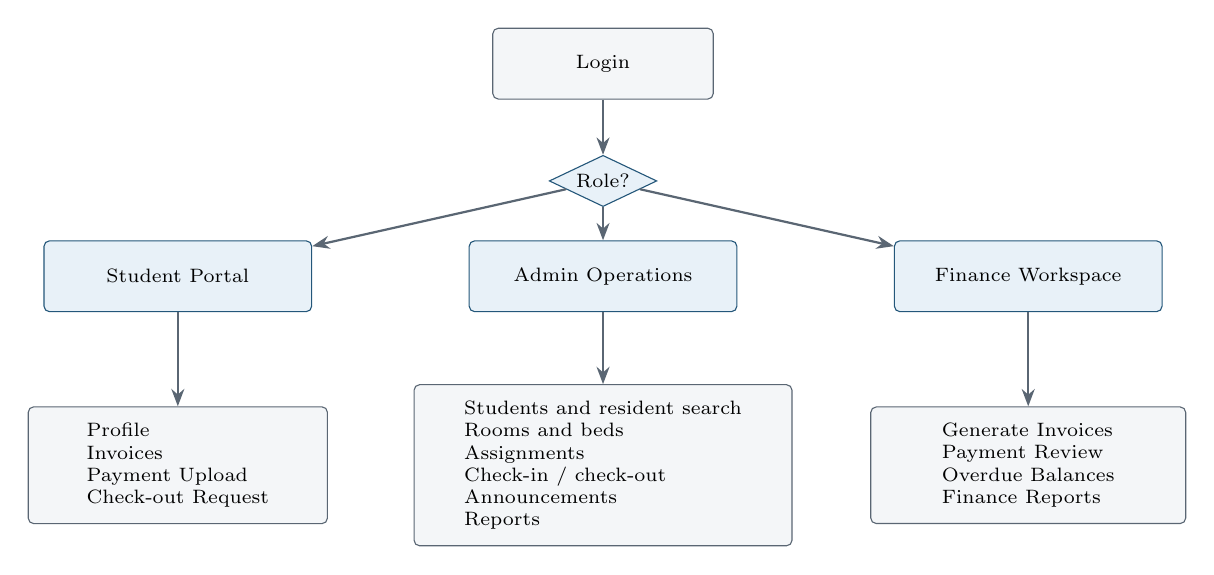
\begin{tikzpicture}[font=\scriptsize, node distance=7mm]
  \node[box, minimum width=28mm] (login) at (7,4.2) {Login};
  \node[decision, below=of login] (role) {Role?};

  \node[module, minimum width=34mm] (student) at (1.6,1.5) {Student Portal};
  \node[module, minimum width=34mm] (admin) at (7,1.5) {Admin Operations};
  \node[module, minimum width=34mm] (finance) at (12.4,1.5) {Finance Workspace};

  \node[box, align=left, minimum width=38mm] (studentPages) at (1.6,-0.9) {
    Profile\\
    Invoices\\
    Payment Upload\\
    Check-out Request};

  \node[box, align=left, minimum width=48mm] (adminPages) at (7,-0.9) {
    Students and resident search\\
    Rooms and beds\\
    Assignments\\
    Check-in / check-out\\
    Announcements\\
    Reports};

  \node[box, align=left, minimum width=40mm] (financePages) at (12.4,-0.9) {
    Generate Invoices\\
    Payment Review\\
    Overdue Balances\\
    Finance Reports};

  \draw[arrow] (login) -- (role);
  \draw[arrow] (role) -- (student);
  \draw[arrow] (role) -- (admin);
  \draw[arrow] (role) -- (finance);
  \draw[arrow] (student) -- (studentPages);
  \draw[arrow] (admin) -- (adminPages);
  \draw[arrow] (finance) -- (financePages);
\end{tikzpicture}%
}
\caption{Role-aware sitemap}
\end{figure}

\subsection{Core User Flow}
The user-flow diagram focuses on the workflows most important to the demo. It shows the role gate after authentication and the main task loops for student payment upload, admin assignment/check-in, admin check-out, and finance confirmation. Each path ends with a status update that is reflected on dashboards and reports.

\begin{figure}[H]
\centering
\resizebox{\textwidth}{!}{%
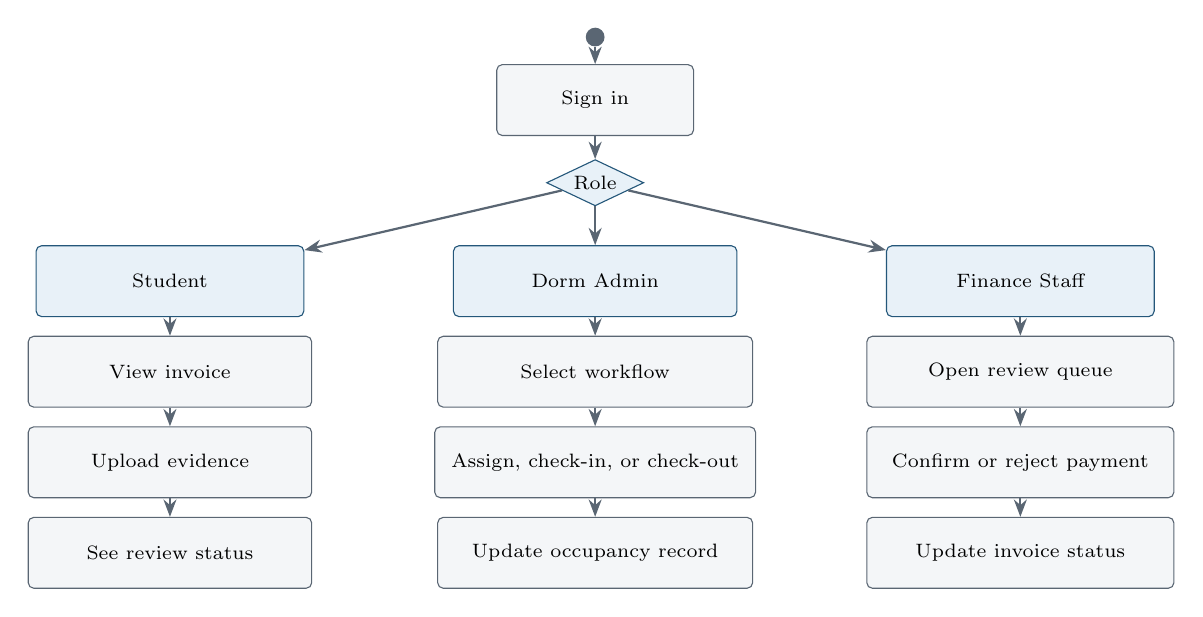
\begin{tikzpicture}[node distance=7mm, font=\scriptsize]
  \node[circle, fill=linegray, inner sep=2.4pt] (start) at (6,5.4) {};
  \node[box, minimum width=25mm] (login) at (6,4.6) {Sign in};
  \node[decision] (role) at (6,3.55) {Role};

  \node[module, minimum width=34mm] (studentRole) at (0.6,2.3) {Student};
  \node[box, minimum width=36mm] (student1) at (0.6,1.15) {View invoice};
  \node[box, minimum width=36mm] (student2) at (0.6,0.0) {Upload evidence};
  \node[box, minimum width=36mm] (student3) at (0.6,-1.15) {See review status};

  \node[module, minimum width=36mm] (adminRole) at (6,2.3) {Dorm Admin};
  \node[box, minimum width=40mm] (admin1) at (6,1.15) {Select workflow};
  \node[box, minimum width=40mm] (admin2) at (6,0.0) {Assign, check-in, or check-out};
  \node[box, minimum width=40mm] (admin3) at (6,-1.15) {Update occupancy record};

  \node[module, minimum width=34mm] (financeRole) at (11.4,2.3) {Finance Staff};
  \node[box, minimum width=39mm] (finance1) at (11.4,1.15) {Open review queue};
  \node[box, minimum width=39mm] (finance2) at (11.4,0.0) {Confirm or reject payment};
  \node[box, minimum width=39mm] (finance3) at (11.4,-1.15) {Update invoice status};

  \draw[arrow] (start) -- (login);
  \draw[arrow] (login) -- (role);
  \draw[arrow] (role) -- (studentRole);
  \draw[arrow] (role) -- (adminRole);
  \draw[arrow] (role) -- (financeRole);
  \draw[arrow] (studentRole) -- (student1);
  \draw[arrow] (student1) -- (student2);
  \draw[arrow] (student2) -- (student3);
  \draw[arrow] (adminRole) -- (admin1);
  \draw[arrow] (admin1) -- (admin2);
  \draw[arrow] (admin2) -- (admin3);
  \draw[arrow] (financeRole) -- (finance1);
  \draw[arrow] (finance1) -- (finance2);
  \draw[arrow] (finance2) -- (finance3);
\end{tikzpicture}%
}
\caption{Core user flow}
\end{figure}

\subsection{Front-end Component Structure}
The front end is server-rendered rather than a single-page application, but it still has a component structure. Reusable Django templates, forms, and HTMX partials act as the front-end components. This structure should be preserved during implementation so that dashboard cards, tables, filters, modals, and status badges are not duplicated across pages. A later React front end could reuse the same service-backed \texttt{/api/v1} endpoints, but it is not required for the local demo.

\begin{figure}[H]
\centering
\resizebox{\textwidth}{!}{%
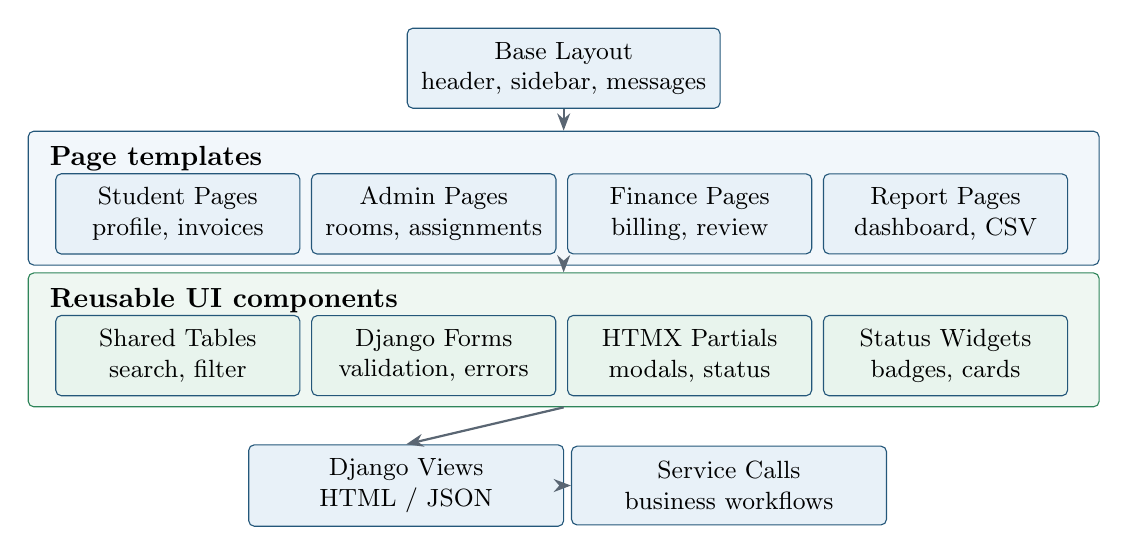
\begin{tikzpicture}[font=\scriptsize]
  \node[componentbox, minimum width=38mm] (base) at (6.5,4.2) {Base Layout\\header, sidebar, messages};
  \node[draw=primary, rounded corners=2pt, fill=softblue!55, minimum width=136mm, minimum height=17mm] (pages) at (6.5,2.55) {};
  \node[anchor=west, font=\bfseries] at (-0.15,3.05) {Page templates};
  \node[componentbox, minimum width=31mm] at (1.6,2.35) {Student Pages\\profile, invoices};
  \node[componentbox, minimum width=31mm] at (4.85,2.35) {Admin Pages\\rooms, assignments};
  \node[componentbox, minimum width=31mm] at (8.1,2.35) {Finance Pages\\billing, review};
  \node[componentbox, minimum width=31mm] at (11.35,2.35) {Report Pages\\dashboard, CSV};

  \node[draw=accent, rounded corners=2pt, fill=softgreen!70, minimum width=136mm, minimum height=17mm] (shared) at (6.5,0.75) {};
  \node[anchor=west, font=\bfseries] at (-0.15,1.25) {Reusable UI components};
  \node[componentbox, minimum width=31mm, fill=softgreen] at (1.6,0.55) {Shared Tables\\search, filter};
  \node[componentbox, minimum width=31mm, fill=softgreen] at (4.85,0.55) {Django Forms\\validation, errors};
  \node[componentbox, minimum width=31mm, fill=softgreen] at (8.1,0.55) {HTMX Partials\\modals, status};
  \node[componentbox, minimum width=31mm, fill=softgreen] at (11.35,0.55) {Status Widgets\\badges, cards};

  \node[componentbox, minimum width=40mm] (views) at (4.5,-1.1) {Django Views\\HTML / JSON};
  \node[componentbox, minimum width=40mm] (api) at (8.6,-1.1) {Service Calls\\business workflows};

  \draw[arrow] (base) -- (pages.north);
  \draw[arrow] (pages.south) -- (shared.north);
  \draw[arrow] (shared.south) -- (views.north);
  \draw[arrow] (views) -- (api);
\end{tikzpicture}%
}
\caption{Front-end component structure}
\end{figure}

\subsection{Screenshot Replacement Plan}
Because the demo has not been implemented yet, this report uses placeholder wireframes instead of invented screenshots. After implementation, the final report should replace the placeholders with real screenshots for the login page, admin dashboard, room assignment screen, student payment upload screen, finance payment review screen, and check-out settlement screen.

\subsection{Dashboard Placeholder}

\begin{figure}[H]
\centering
\resizebox{\textwidth}{!}{%
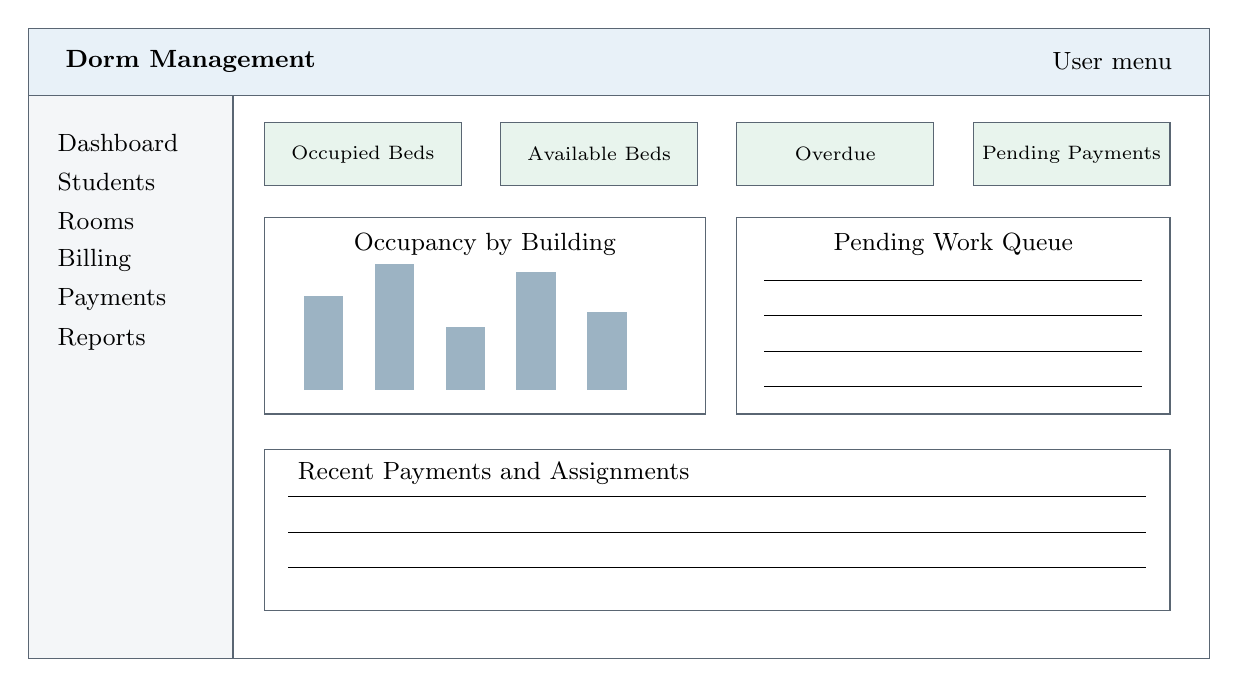
\begin{tikzpicture}[font=\small]
  \draw[draw=linegray, fill=white] (0,0) rectangle (15,8);
  \draw[fill=softblue, draw=linegray] (0,7.15) rectangle (15,8);
  \node[anchor=west] at (0.35,7.58) {\textbf{Dorm Management}};
  \node[anchor=east] at (14.65,7.58) {User menu};

  \draw[fill=softgray, draw=linegray] (0,0) rectangle (2.6,7.15);
  \node[anchor=west] at (0.25,6.55) {Dashboard};
  \node[anchor=west] at (0.25,6.05) {Students};
  \node[anchor=west] at (0.25,5.55) {Rooms};
  \node[anchor=west] at (0.25,5.05) {Billing};
  \node[anchor=west] at (0.25,4.55) {Payments};
  \node[anchor=west] at (0.25,4.05) {Reports};

  \foreach \x/\label in {3.0/Occupied Beds,6.0/Available Beds,9.0/Overdue,12.0/Pending Payments} {
    \draw[fill=softgreen, draw=linegray] (\x,6.0) rectangle ++(2.5,0.8);
    \node[font=\scriptsize] at (\x+1.25,6.4) {\label};
  }

  \draw[fill=white, draw=linegray] (3.0,3.1) rectangle (8.6,5.6);
  \node at (5.8,5.25) {Occupancy by Building};
  \draw[fill=primary!45, draw=none] (3.5,3.4) rectangle (4.0,4.6);
  \draw[fill=primary!45, draw=none] (4.4,3.4) rectangle (4.9,5.0);
  \draw[fill=primary!45, draw=none] (5.3,3.4) rectangle (5.8,4.2);
  \draw[fill=primary!45, draw=none] (6.2,3.4) rectangle (6.7,4.9);
  \draw[fill=primary!45, draw=none] (7.1,3.4) rectangle (7.6,4.4);

  \draw[fill=white, draw=linegray] (9.0,3.1) rectangle (14.5,5.6);
  \node at (11.75,5.25) {Pending Work Queue};
  \draw (9.35,4.8) -- (14.15,4.8);
  \draw (9.35,4.35) -- (14.15,4.35);
  \draw (9.35,3.9) -- (14.15,3.9);
  \draw (9.35,3.45) -- (14.15,3.45);

  \draw[fill=white, draw=linegray] (3.0,0.6) rectangle (14.5,2.65);
  \node[anchor=west] at (3.3,2.35) {Recent Payments and Assignments};
  \draw (3.3,2.05) -- (14.2,2.05);
  \draw (3.3,1.6) -- (14.2,1.6);
  \draw (3.3,1.15) -- (14.2,1.15);
\end{tikzpicture}%
}
\caption{Administrative dashboard placeholder wireframe}
\end{figure}

\subsection{Payment Review Placeholder}

\begin{figure}[H]
\centering
\resizebox{0.95\textwidth}{!}{%
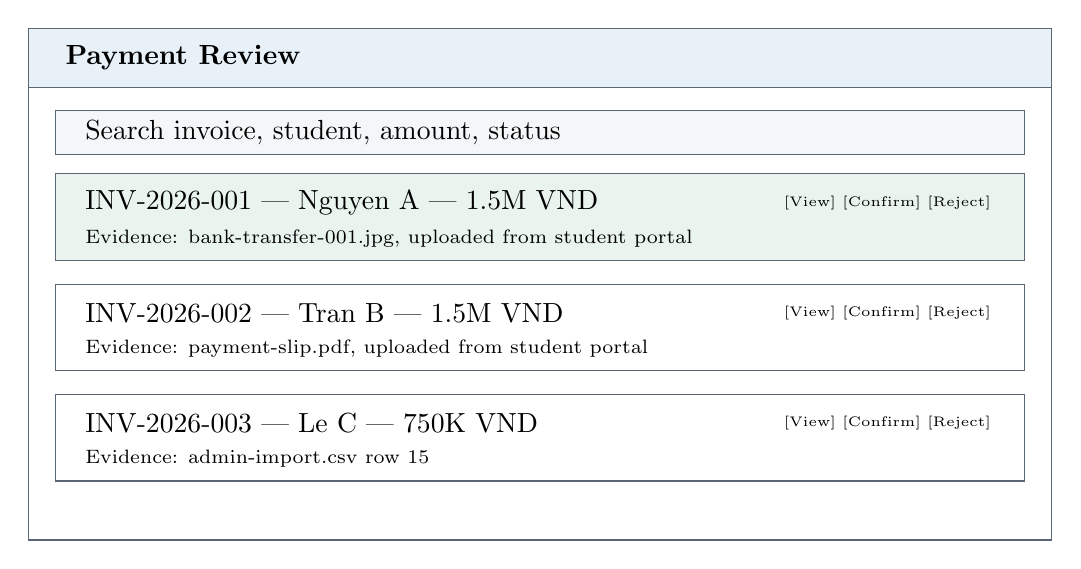
\begin{tikzpicture}
  \draw[draw=linegray, fill=white] (0,0) rectangle (13,6.5);
  \draw[fill=softblue, draw=linegray] (0,5.75) rectangle (13,6.5);
  \node[anchor=west] at (0.35,6.13) {\textbf{Payment Review}};
  \draw[fill=softgray, draw=linegray] (0.35,4.9) rectangle (12.65,5.45);
  \node[anchor=west] at (0.6,5.18) {Search invoice, student, amount, status};

  \draw[fill=softgreen, draw=linegray] (0.35,3.55) rectangle (12.65,4.65);
  \node[anchor=west] at (0.6,4.28) {INV-2026-001  |  Nguyen A  |  1.5M VND};
  \node[anchor=east, font=\tiny] at (12.35,4.28) {[View] [Confirm] [Reject]};
  \node[anchor=west, font=\scriptsize] at (0.6,3.83) {Evidence: bank-transfer-001.jpg, uploaded from student portal};

  \draw[fill=white, draw=linegray] (0.35,2.15) rectangle (12.65,3.25);
  \node[anchor=west] at (0.6,2.88) {INV-2026-002  |  Tran B  |  1.5M VND};
  \node[anchor=east, font=\tiny] at (12.35,2.88) {[View] [Confirm] [Reject]};
  \node[anchor=west, font=\scriptsize] at (0.6,2.43) {Evidence: payment-slip.pdf, uploaded from student portal};

  \draw[fill=white, draw=linegray] (0.35,0.75) rectangle (12.65,1.85);
  \node[anchor=west] at (0.6,1.48) {INV-2026-003  |  Le C  |  750K VND};
  \node[anchor=east, font=\tiny] at (12.35,1.48) {[View] [Confirm] [Reject]};
  \node[anchor=west, font=\scriptsize] at (0.6,1.03) {Evidence: admin-import.csv row 15};
\end{tikzpicture}%
}
\caption{Payment review placeholder wireframe}
\end{figure}

\subsection{API Design}
The MVP is primarily server-rendered, so user-facing navigation uses HTML routes such as \texttt{/students/}, \texttt{/rooms/}, and \texttt{/payments/review/}. The API contract is documented separately as REST-style JSON endpoints for asynchronous widgets, dashboard data, recommendations, and future integration. The API follows the project convention: plural resource names, kebab-case for multi-word resources, JSON bodies, consistent status codes, and versioned URLs under \texttt{/api/v1}. All endpoints require authentication unless explicitly marked public.

\begin{longtable}{L{0.11\textwidth} L{0.34\textwidth} L{0.30\textwidth} L{0.12\textwidth}}
\toprule
\textbf{Method} & \textbf{Endpoint} & \textbf{Purpose} & \textbf{Role}\\
\midrule
\endhead
GET & \path|/api/v1/dashboard-summary| & Dashboard counts and queue summaries. & Staff\\
GET & \path|/api/v1/students| & Search and paginate students. & Admin\\
POST & \path|/api/v1/students| & Create a student record. & Admin\\
GET & \path|/api/v1/rooms| & List rooms, filters, and occupancy. & Admin\\
GET & \path|/api/v1/beds?status=available| & List available beds. & Admin\\
POST & \path|/api/v1/assignment-recommendations| & Return ranked beds for a student. & Admin\\
POST & \path|/api/v1/assignments| & Reserve or activate a bed assignment. & Admin\\
POST & \path|/api/v1/assignments/{assignmentId}/check-in| & Finalize check-in. & Admin\\
POST & \path|/api/v1/assignments/{assignmentId}/check-out| & Complete check-out settlement. & Admin\\
POST & \path|/api/v1/invoices/batches| & Generate recurring invoices. & Finance\\
GET & \path|/api/v1/students/me/invoices| & Student invoice list. & Student\\
POST & \path|/api/v1/payments| & Upload payment evidence. & Student\\
POST & \path|/api/v1/payments/{paymentId}/confirm| & Confirm a pending payment. & Finance\\
POST & \path|/api/v1/payments/{paymentId}/reject| & Reject a pending payment. & Finance\\
POST & \path|/api/v1/announcements| & Create announcement. & Admin\\
GET & \path|/api/v1/reports/occupancy| & Return occupancy report data or CSV. & Staff\\
\bottomrule
\end{longtable}

Responses use a consistent envelope:
\begin{verbatim}
{
  "success": true,
  "message": "Operation completed.",
  "data": {}
}
\end{verbatim}

Validation errors return \texttt{400 Bad Request} or \texttt{422 Unprocessable Entity}; authorization failures return \texttt{401 Unauthorized} or \texttt{403 Forbidden}; business conflicts such as double booking return \texttt{409 Conflict}.

\subsection{Representative API Payloads}
The final implementation may render most interactions as HTML, but the following JSON shapes define the data contract for the workflows that benefit from asynchronous responses.

\textbf{Assignment recommendation request and response}:
\begin{verbatim}
POST /api/v1/assignment-recommendations
{
  "studentId": 42,
  "preferences": {
    "buildingId": 2,
    "floorPreference": "low",
    "roomType": "shared"
  },
  "limit": 5
}

200 OK
{
  "success": true,
  "message": "Recommendations generated.",
  "data": {
  "studentId": 42,
  "candidates": [
    {
      "bedId": 311,
      "building": "A",
      "room": "A-203",
      "bedCode": "A-203-B",
      "availableBedsInRoom": 1,
      "policyMatch": true,
      "score": 86,
      "reasons": ["gender policy match", "preferred building"]
    }
  ]
  }
}
\end{verbatim}

\textbf{Payment evidence upload result}:
\begin{verbatim}
POST /api/v1/payments
Content-Type: multipart/form-data
fields: invoiceId, amount, evidenceFiles[]

201 Created
{
  "success": true,
  "message": "Payment evidence submitted for finance review.",
  "data": {
  "paymentId": 88,
  "invoiceId": 1204,
  "status": "pending_review",
  "evidenceCount": 2
  }
}
\end{verbatim}

\subsection{Input and Output Formats}
\begin{itemize}
  \item HTML forms are used for most CRUD workflows.
  \item JSON responses are used for recommendation results, dashboard widgets, and HTMX status responses.
  \item CSV import/export is used for student imports and report downloads.
  \item Uploaded payment evidence accepts common image and PDF formats with file size limits.
  \item Email messages are generated as plain text and HTML summaries for reminders and payment review digests.
\end{itemize}

\subsection{External Interfaces}
\begin{itemize}
  \item \textbf{Email service}: sends invoice reminders, payment review summaries, and announcements.
  \item \textbf{File storage}: stores payment evidence and inspection attachments.
  \item \textbf{Future payment gateway}: can replace or supplement manual payment evidence review.
  \item \textbf{Future university SSO}: can replace local user authentication while preserving role permissions.
\end{itemize}

\section{Component-Level / Detailed Design}

\subsection{Service Method Map}
The service layer is the implementation boundary for workflow logic. The following table lists the main service classes that should exist in code and the method names the implementation can start from.

\begin{longtable}{L{0.28\textwidth} L{0.33\textwidth} L{0.26\textwidth}}
\toprule
\textbf{Service Class} & \textbf{Core Methods} & \textbf{Primary Dependencies}\\
\midrule
\endhead
\texttt{IdentityService} & \texttt{require\_role}, \texttt{can\_view\_student}, \texttt{get\_profile} & Django auth, UserProfile, Student\\
\texttt{ResidentService} & \texttt{create\_student}, \texttt{import\_students}, \texttt{get\_resident\_history} & Student, Assignment, Invoice\\
\texttt{RoomInventoryService} & \texttt{create\_room}, \texttt{sync\_beds}, \texttt{set\_bed\_status} & Building, Floor, Room, Bed\\
\texttt{AssignmentService} & \texttt{recommend\_beds}, \texttt{reserve\_bed}, \texttt{activate\_assignment}, \texttt{transfer\_student} & Student, Bed, Assignment, AuditLog\\
\texttt{CheckoutService} & \texttt{finalize\_checkin}, \texttt{settle\_checkout}, \texttt{calculate\_damage\_fee} & Assignment, Inspection, InvoiceLine\\
\texttt{BillingService} & \texttt{generate\_initial\_invoice}, \texttt{generate\_recurring\_rent}, \texttt{calculate\_invoice\_balance} & Invoice, InvoiceLine, Payment\\
\texttt{PaymentReviewService} & \texttt{submit\_payment\_evidence}, \texttt{send\_review\_digest}, \texttt{confirm\_payment}, \texttt{reject\_payment} & Payment, PaymentEvidence, FileStorage, NotificationService\\
\texttt{NotificationService} & \texttt{send\_announcement}, \texttt{send\_invoice\_reminder}, \texttt{record\_notification} & Announcement, Notification, EmailGateway\\
\texttt{ReportingService} & \texttt{dashboard\_summary}, \texttt{occupancy\_report}, \texttt{finance\_report} & Querysets, aggregates, CSV exporter\\
\bottomrule
\end{longtable}

\subsection{Identity and Access Module}
\textbf{Responsibilities}: authenticate users, map users to roles, protect views, and expose role-aware navigation.

\textbf{Key methods and functions}:
\begin{itemize}
  \item \texttt{require\_role(user, roles)}: checks whether the current user has one of the allowed roles.
  \item \texttt{get\_profile(user)}: returns profile and role information.
  \item \texttt{can\_view\_student(user, student)}: enforces student self-access and staff access.
\end{itemize}

\textbf{Dependencies}: Django auth, UserProfile, Student.

\subsection{Resident Management Module}
\textbf{Responsibilities}: manage student records, contact details, status, and resident history.

\textbf{Key methods and functions}:
\begin{itemize}
  \item \texttt{create\_student(data)}: validates uniqueness and creates a student record.
  \item \texttt{import\_students(csv\_file)}: validates and imports student data from CSV.
  \item \texttt{get\_resident\_history(student)}: returns assignments, invoices, and check-in/check-out records.
\end{itemize}

\textbf{Internal logic}: student status changes are controlled by workflow events. For example, check-in can change a student from applicant to active, while completed check-out can change active to checked\_out.

\subsection{Room Inventory Module}
\textbf{Responsibilities}: manage buildings, floors, rooms, beds, capacity, and bed lifecycle state.

\textbf{Key methods and functions}:
\begin{itemize}
  \item \texttt{create\_room(floor, room\_number, capacity, policy)}.
  \item \texttt{sync\_beds(room, capacity)}: creates missing bed records when capacity changes.
  \item \texttt{set\_bed\_status(bed, status, reason)}: validates legal transitions and logs changes.
\end{itemize}

\textbf{Dependencies}: Building, Floor, Room, Bed, AuditLog.

\subsection{Assignment Module}
\textbf{Responsibilities}: recommend beds, reserve beds, activate assignments, transfer students, and maintain occupancy history.

\textbf{Room assignment pseudocode}:

\begin{verbatim}
function recommend_beds(student, preferences, limit):
    candidates = query beds where status = "available"
    candidates = exclude rooms with inactive or maintenance status

    for each candidate in candidates:
        score = 0
        if room gender_policy matches student gender:
            score += 40
        else if room gender_policy is "mixed" or "unspecified":
            score += 15
        else:
            continue

        score += capacity_score(room.available_bed_count)
        score += preference_score(candidate, preferences)
        score -= distance_penalty(candidate, preferences)

        candidate.score = score

    sort candidates by score descending, building, room_number, bed_code
    return first limit candidates

function reserve_bed(student, bed, actor):
    begin transaction
        lock selected bed row
        if bed.status is not "available":
            raise AssignmentConflict
        cancel previous active reservation for student if any
        create assignment with status = "reserved"
        set bed.status = "reserved"
        write audit log
    commit transaction
\end{verbatim}

\textbf{Consistency rules}:
\begin{itemize}
  \item A student may have at most one active or reserved assignment.
  \item A bed may have at most one active or reserved assignment.
  \item Reservation and activation must lock the bed row to avoid double booking.
  \item Manual overrides require an admin reason.
\end{itemize}

\subsection{Check-In / Check-Out Module}
\textbf{Responsibilities}: finalize move-in, record handover condition, process departure, record inspection, calculate penalties, release bed inventory, and settle deposits.

\textbf{Check-out pseudocode}:

\begin{verbatim}
function settle_checkout(assignment, inspection_data, actor):
    begin transaction
        assert assignment.status == "active"
        create checkout inspection from inspection_data
        penalty = calculate_damage_fee(inspection_data)
        unpaid = calculate_outstanding_balance(assignment.student)
        if penalty > 0:
            create penalty invoice line
        update deposit settlement using penalty and unpaid amount
        assignment.status = "completed"
        assignment.end_date = today
        if inspection requires cleaning:
            bed.status = "cleaning"
        else:
            bed.status = "available"
        student.status = "checked_out"
        write audit log
    commit transaction
\end{verbatim}

\subsection{Billing Module}
\textbf{Responsibilities}: generate invoices, invoice lines, deposits, fees, rent cycles, penalties, and balances.

\textbf{Key methods and functions}:
\begin{itemize}
  \item \texttt{generate\_initial\_invoice(student, assignment)}.
  \item \texttt{generate\_recurring\_rent(period)}.
  \item \texttt{calculate\_invoice\_balance(invoice)}.
  \item \texttt{mark\_overdue\_invoices(today)}.
\end{itemize}

\textbf{Internal logic}: invoice status is derived from due date and confirmed payment total. Pending payments do not reduce outstanding balance until confirmed.

\subsection{Payment Review Module}
\textbf{Responsibilities}: accept payment evidence, group pending submissions, send review emails, confirm or reject payments, update invoice status, and log decisions.

\textbf{Payment evidence aggregation pseudocode}:

\begin{verbatim}
function submit_payment_evidence(invoice, amount, files, student):
    begin transaction
        assert invoice belongs to student
        payment = create payment(status="pending_review", amount=amount)
        for file in files:
            validate file type and size
            store file and create payment evidence
        enqueue payment_review_digest(payment)
    commit transaction

function send_payment_review_digest():
    pending = query payments where status = "pending_review"
              and review_email_sent = false
    grouped = group pending by finance recipient or dorm building
    for each group in grouped:
        render email with invoice, student, amount, and evidence links
        send email
        mark payments as review_email_sent

function confirm_payment(payment, actor):
    begin transaction
        lock payment and invoice
        assert actor has finance permission
        payment.status = "confirmed"
        payment.reviewed_by = actor
        update invoice status from confirmed payment total
        write audit log
    commit transaction
\end{verbatim}

\subsection{Notification Module}
\textbf{Responsibilities}: send announcements, invoice reminders, overdue notices, and payment review emails.

\textbf{Key methods and functions}:
\begin{itemize}
  \item \texttt{send\_announcement(announcement)}.
  \item \texttt{send\_invoice\_reminder(invoice)}.
  \item \texttt{send\_payment\_review\_digest(payments)}.
  \item \texttt{record\_notification(recipient, channel, status)}.
\end{itemize}

\subsection{Reporting Module}
\textbf{Responsibilities}: produce dashboard metrics and exportable reports.

\textbf{Example dashboard queries}:
\begin{itemize}
  \item Count beds by status and building.
  \item Count active students and pending check-ins.
  \item Sum outstanding invoice amounts by due-date bucket.
  \item List pending payment reviews with age in days.
\end{itemize}

\subsection{Demo Data Module}
\textbf{Responsibilities}: seed a realistic demo dataset that supports the presentation scenario.

\textbf{Generated data}:
\begin{itemize}
  \item Buildings, floors, rooms, and beds with mixed availability.
  \item Student accounts with active, applicant, checked-out, and suspended statuses.
  \item Assignments in reserved, active, and completed states.
  \item Invoices with paid, overdue, partially paid, and pending review statuses.
  \item Payment evidence records and announcement examples.
\end{itemize}

\section{Quality Attributes and Design Rationale}

\begin{longtable}{L{0.18\textwidth} L{0.62\textwidth} L{0.12\textwidth}}
\toprule
\textbf{Attribute} & \textbf{Design Support} & \textbf{Priority}\\
\midrule
\endhead
Maintainability & Django apps separate identity, residents, rooms, assignments, billing, payments, notifications, and reports. Service classes keep workflow rules out of views. & High\\
Scalability & PostgreSQL indexes support larger student and invoice tables. The architecture can move email sending to background jobs later. & Medium\\
Security & Authentication, role groups, permission checks, file validation, audit logs, and restricted student self-access protect sensitive data. & High\\
Reliability & Assignment and payment operations use transactions and row locks for critical state changes. & High\\
Usability & Role-focused dashboards, searchable tables, clear workflow queues, and status labels reduce staff effort. & High\\
Performance & Server-side filtering, pagination, database indexes, and aggregate dashboard queries keep pages responsive. & Medium\\
Extensibility & External integrations are isolated behind services, allowing future payment gateway, SSO, and mobile clients. & Medium\\
Auditability & Critical financial and occupancy actions write audit entries with actor, timestamp, target, and change details. & High\\
\bottomrule
\end{longtable}

\section{Requirement--Design Traceability}

\begin{longtable}{L{0.10\textwidth} L{0.25\textwidth} L{0.37\textwidth} L{0.17\textwidth}}
\toprule
\textbf{Req. ID} & \textbf{Requirement} & \textbf{Design Element} & \textbf{Verification Target}\\
\midrule
\endhead
FR-01 & Authentication and roles & Identity and Access module, Django auth, UserProfile, role groups, permission decorators. & Login and role-access tests.\\
FR-02 & Student profile management & Resident Management module, Student model, student CRUD views. & CRUD and import tests.\\
FR-03 & Room and bed inventory & Room Inventory module, Building, Floor, Room, and Bed models. & Room/bed CRUD tests.\\
FR-04 & Automatic assignment & Assignment service, scoring strategy, AssignmentCandidate structure. & Scoring rule tests.\\
FR-05 & Manual assignment override & Assignment service, admin views, audit log reason field. & Override workflow test.\\
FR-06 & Check-in workflow & Check-In / Check-Out module, Assignment state change, Inspection model. & Check-in integration test.\\
FR-07 & Check-out workflow & Check-In / Check-Out module, checkout settlement algorithm, penalty invoice lines. & Checkout settlement test.\\
FR-08 & Billing and invoices & Billing module, Invoice and InvoiceLine models. & Invoice generation test.\\
FR-09 & Payment evidence upload & Payment Review module, PaymentEvidence model, file storage gateway. & Upload and validation test.\\
FR-10 & Payment review and confirmation & Payment review service, email digest, confirmation transaction, audit log. & Confirm/reject tests.\\
FR-11 & Notifications and announcements & Notification module, Announcement and Notification models. & Notification delivery test.\\
FR-12 & Dashboard and reports & Reporting module, dashboard queries, CSV report endpoints. & Aggregate report tests.\\
FR-13 & Audit trail & AuditLog model and service-level audit writing. & Audit record assertions.\\
FR-14 & Synthetic demo data & Demo Data module and seed command. & Seed command test.\\
NFR-01 & Security & Authentication middleware, role checks, restricted file access, file validation. & Negative access tests.\\
NFR-02 & Reliability & Database transactions, row locks, model constraints. & Concurrency test.\\
NFR-03 & Usability & Role-focused navigation, placeholder wireframes, searchable lists. & Demo task walkthrough.\\
NFR-04 & Performance & Pagination, indexes, aggregate queries. & Query-count and timing checks.\\
NFR-05 & Maintainability & App modularization, service layer, design patterns. & Design review.\\
NFR-06 & Extensibility & Integration gateways and strategy interfaces. & Extension review.\\
NFR-07 & Auditability & AuditLog and payment/assignment decision tracking. & Audit trail tests.\\
NFR-08 & Portability & Environment variables and Docker-ready deployment design. & Fresh setup run.\\
\bottomrule
\end{longtable}

\section{Validation / Testing Strategy}

\subsection{Design Review}
The design should be reviewed against the original project objectives, MVP scope, and traceability matrix. Reviewers should verify that every major workflow has a responsible module, data model, user interface path, and test strategy. The review checklist should include:
\begin{itemize}
  \item Each diagram uses the correct notation for its purpose: use cases inside a system boundary, UML activity and state symbols, DFD processes/data stores/external entities, and ERD cardinalities.
  \item No rendered diagram has overlapping text, crossed labels, or unreadable connector labels.
  \item Every entity relationship in the ERD has an explicit cardinality such as 1:1, 1:N, or N:M through an associative entity.
  \item Each lifecycle state transition is represented in both the state diagram and the service-level pseudocode.
  \item UI figures remain labelled as placeholders until replaced with real screenshots from the working demo.
\end{itemize}

\subsection{Test Plan Overview}

\begin{longtable}{L{0.20\textwidth} L{0.45\textwidth} L{0.22\textwidth}}
\toprule
\textbf{Test Area} & \textbf{Focus} & \textbf{Method}\\
\midrule
\endhead
Unit tests & Service functions, status transitions, balance calculations, scoring rules. & Django test cases.\\
Integration tests & Assignment, check-in, billing, payment confirmation, check-out settlement. & Database-backed tests.\\
Permission tests & Role access for student, admin, finance, and system administrator. & View and API tests.\\
UI tests & Core workflows through browser pages. & Manual demo script or browser automation.\\
Data tests & Seed data consistency and report totals. & Management command tests.\\
Security tests & Unauthorized access, file type rejection, cross-user data access. & Negative tests.\\
\bottomrule
\end{longtable}

\subsection{Key Test Cases}
\begin{enumerate}
  \item Student can sign in and view only their own assignment and invoices.
  \item Admin creates a room with four beds and sees all beds in available status.
  \item Assignment recommendation excludes occupied, inactive, and gender-incompatible rooms.
  \item Two admins cannot reserve the same bed at the same time.
  \item Check-in changes assignment to active and bed to occupied.
  \item Finance generates an invoice and student uploads payment evidence.
  \item Payment upload creates pending payment, stores evidence, and queues review email.
  \item Finance confirms payment and invoice status changes to paid when the confirmed amount is sufficient.
  \item Rejected payment does not reduce outstanding invoice balance.
  \item Check-out inspection creates penalties, settles deposit, completes assignment, and releases bed.
  \item Dashboard counts match database records after seed data is loaded.
  \item Unauthorized users cannot access staff pages or payment confirmation endpoints.
\end{enumerate}

\subsection{Acceptance Criteria}
\begin{itemize}
  \item The demo can be started from a clean database with synthetic data.
  \item Student, admin, and finance accounts can complete their main workflows.
  \item The system prevents double booking and unauthorized payment confirmation.
  \item Dashboard metrics update after assignment, payment, and check-out actions.
  \item Payment evidence review includes email notification and manual confirmation.
  \item The report and implementation remain aligned through the traceability matrix.
\end{itemize}

\section{Conclusion}
The proposed Student Dormitory Management System provides a practical MVP design for digitizing dormitory operations. The design centralizes student records, room and bed inventory, occupancy workflows, billing, payment review, announcements, notifications, reporting, and demo data generation. The expected benefit is a single source of operational truth: dorm staff can see current occupancy, finance staff can trace invoices and payment evidence, and students can view assignments and payment status without relying on separate spreadsheets or messages.

The report is ready to guide implementation because each major requirement is connected to an architecture layer, data model, interface path, service method, and verification target. The most important correctness risks, including bed double booking, unauthorized payment confirmation, invalid lifecycle transitions, and lost audit evidence, are handled through role permissions, service-layer transactions, database constraints, and audit logging.

For the project demo, the server-rendered Django stack is deliberately practical. It can run locally with Docker Compose, PostgreSQL, seeded demo data, local media storage, and a console or SMTP email backend. The same structure can later move to a low-cost VM or container host with managed PostgreSQL, S3-compatible media storage, TLS at a reverse proxy, and environment-based configuration. Future improvements can add a payment gateway, university SSO, online housing applications, roommate matching, visitor management, background job processing, mobile access, and a separate React or mobile client using the documented \texttt{/api/v1} endpoints.

\end{document}
